\documentclass[9pt]{beamer}

%%% INÍCIO DE PACOTES %%%

\usepackage[brazilian]{babel}
\usepackage[utf8]{inputenc}

\usepackage{graphicx} % Possibilita inclusão de imagem
\usepackage{tikz} % Permite desenhar
\usetikzlibrary{patterns} % Permite hachurar áreas
\usepackage{pgfplots} % Com tikz, desenha gráfico
\usetikzlibrary{decorations.pathreplacing, angles, quotes} % Permite desenhar "chaves"
\usepackage{mathtools, amsthm, amssymb, amsbsy} % Pacotes de Matemática
\usepackage{colonequals} % Símbolo de definição: \colonequals ou \equalscolon
\usepackage{hyperref} % Link para partes do próprio texto
\usepackage{lmodern} % Melhora a fonte
\usepackage{ragged2e}
\usepackage{xcolor}

\apptocmd{\frame}{}{\justifying}{} % Allow optional arguments after frame.

%%% INÍCIO DE APARÊNCIA %%%
\usetheme[]{metropolis}
\usecolortheme[]{wolverine}

\definecolor{MyRed}{RGB}{226, 3, 52}
\definecolor{MyGreen}{RGB}{0, 153, 73}
\definecolor{MyBlue}{RGB}{0, 84, 154}
\definecolor{MyOrange}{RGB}{239, 130, 6}

\definecolor{YellowBar}{RGB}{254, 231, 2}
\definecolor{YellowSecondaryBar}{RGB}{251, 199, 7}
\definecolor{MyBG}{RGB}{250, 250, 250}

\setbeamercolor{MC}{bg = MyBG}

\usefonttheme{serif}
\setbeamersize{text margin left = 9pt,text margin right = 9pt} 
\setbeamercovered{transparent = 0.5}

\setbeamertemplate{footline}{% Formatação do rodaé de todos os slides
	\leavevmode%
	\hbox{%
		\begin{beamercolorbox}[wd = 0.800\textwidth, ht = 4ex, dp = 2ex, left]{MC}%
			\usebeamerfont{author in head/foot}\texttt{\hspace{9pt}\insertshortauthor~|~\insertshorttitle.}%
		\end{beamercolorbox}%
		\begin{beamercolorbox}[wd = 0.120\textwidth, ht = 4ex, dp = 2ex, center]{MC}%
			\raisebox{-2pt}{\insertslidenavigationsymbol~\insertsectionnavigationsymbol}%
		\end{beamercolorbox}%
		\begin{beamercolorbox}[wd = 0.080\textwidth, ht = 4ex, dp = 2ex, center]{MC}%
			\usebeamerfont{date in head/foot}\texttt{\insertframenumber~/~\inserttotalframenumber}%
		\end{beamercolorbox}%
	}%
}

\setbeamertemplate{theorems}[numbered] % habilita numeração nos teoremas, definições, etc.

%%% INÍCIO CÓDIGO ADICIONAL %%%

\theoremstyle{definition} % retira a formatação do texto (o padrão é 'plain')

\newtheorem{mydef}{Definição}
\newtheorem*{mydef*}{Definição}
\newtheorem{mythm}{Teorema}
\newtheorem*{mythm*}{Teorema}
\newtheorem{myobs}{Observação}
\newtheorem*{myobs*}{Observação}
\newtheorem{myexp}{Exemplo}
\newtheorem*{myexp*}{Exemplo}
\newtheorem{mypro}{Proposição}
\newtheorem*{mypro*}{Proposição}
\newtheorem{mycol}{Corolário}
\newtheorem*{mycol*}{Corolário}
\newtheorem{mylem}{Lema}
\newtheorem*{mylem*}{Lema}

%%% INÍCIO DA DEFINIÇÃO DE NOVOS SÍMBOLOS E FUNÇÕES %%%

\DeclareMathOperator{\PX}{\mathbb{P}} % Probability symbol
\DeclareMathOperator{\EX}{\mathbb{E}} % Expectation symbol \mathbbmss
\DeclareMathOperator{\VX}{\mathbb{V}} % Variance symbol
\DeclareMathOperator{\FX}{\mathcal{F}} % Sigma-algebra symbol
\DeclareMathOperator{\AX}{\mathcal{A}} % Sigma-algebra symbol
\DeclareMathOperator{\NX}{\mathbb{N}} % Natural set symbol
\DeclareMathOperator{\ZX}{\mathbb{Z}} % Integer set symbol
\DeclareMathOperator{\QX}{\mathbb{Q}} % Rational set symbol
\DeclareMathOperator{\IX}{\mathbb{I}} % Irrational set symbol
\DeclareMathOperator{\RX}{\mathbb{R}} % Real set symbol
\DeclareMathOperator{\CX}{\mathbb{C}} % Complex set symbol
\DeclareMathOperator{\LX}{\mathbb{L}} % Lattice set symbol
\DeclareMathOperator{\PL}{\mathcal{P}} % Lattice set symbol
\DeclareMathOperator{\GX}{\mathcal{G}} % Group symbol
\DeclareMathOperator{\HC}{\mathcal{H}} % Horizontal crossing
\DeclareMathOperator{\VC}{\mathcal{V}} % Vertical crossing
\DeclareMathOperator{\HL}{\mathcal{H}} % Horizontal crossing
\DeclareMathOperator{\VL}{\mathcal{V}} % Vertical crossing
\newcommand{\diff}{{\nabla_i}f(\omega)}
\newcommand{\diffe}{{\nabla_e}f(\omega)}
\newcommand{\flip}{\text{Flip}_i(\omega)}
\newcommand{\flipe}{\text{Flip}_e(\omega)}
\newcommand{\infl}{\text{Inf}_i(f(\omega))}
\newcommand{\infle}{\text{Inf}_e(f(\omega))}

\makeatletter % Define função ERF
\pgfmathdeclarefunction{erf}{1}{%
	\begingroup
	\pgfmathparse{#1 > 0 ? 1 : -1}%
	\edef\sign{\pgfmathresult}%
	\pgfmathparse{abs(#1)}%
	\edef\x{\pgfmathresult}%
	\pgfmathparse{1/(1+0.3275911*\x)}%
	\edef\t{\pgfmathresult}%
	\pgfmathparse{%
		1 - (((((1.061405429*\t -1.453152027)*\t) + 1.421413741)*\t 
		-0.284496736)*\t + 0.254829592)*\t*exp(-(\x*\x))}%
	\edef\y{\pgfmathresult}%
	\pgfmathparse{(\sign)*\y}%
	\pgfmath@smuggleone\pgfmathresult%
	\endgroup
}
\makeatother

\newenvironment{myitemize}
{ \begin{itemize}
	\setlength{\itemsep}{6pt}
	\setlength{\parskip}{0pt}
	\setlength{\parsep}{0pt} }
{ \end{itemize} } 

%\setbeamerfont{bibliography item}{size=\small}
%\setbeamerfont{bibliography entry author}{size=\small}
%\setbeamerfont{bibliography entry title}{size=\small}
%\setbeamerfont{bibliography entry location}{size=\small}
%\setbeamerfont{bibliography entry note}{size=\small}

\setbeamertemplate{frametitle continuation}{} 

%%% INÍCIO DAS INFORMAÇÕES %%%

\title{Transição de Fase em Modelos de Percolação via Funções Booleanas}
\author[André V. R. Amaral]{André Victor Ribeiro Amaral}

\begin{document}
	\AtBeginSection{} % Elimina slide inicial de cada seção
	\metroset{block = fill} % Permite que os blocos de teoremas tenham cor de fundo e estrutura
	
	\begin{frame}[t]
		\centering
		\vspace{40pt}
		\texttt{{\Large \usebeamercolor[fg]{frametitle} Transição de Fase em Modelos de Percolação via \\ Funções Booleanas}} \\
		\vspace{26pt}
		\texttt{{\normalsize André Victor Ribeiro Amaral${}^{\dagger}$}} \\
		\texttt{{\small Orientador$:$ Roger William Câmara Silva}}\\
		\vspace{26pt}
		\texttt{{\normalsize \usebeamercolor[fg]{frametitle} Defesa do Trabalho de Dissertação}} \\
		\vspace{26pt}
		\texttt{{\small Universidade Federal de Minas Gerais $-$ ICEx, Departamento de Estatística.}}\\
		\texttt{{\small (10/08/2020)}} \\
		\vspace{26pt}
		\begin{flushleft} \texttt{{\scriptsize ${}^{\dagger}$~E-mail$:$ \href{mailto:avramaral@gmail.com}{avramaral@gmail.com}}} \end{flushleft}
		
	\end{frame}

	\begin{frame}[t]
		\frametitle{Sumário}
		\tableofcontents
	\end{frame}

	\section{Introdução}
	\begin{frame}[t]
		\frametitle{Introdução}	
		Em modelos com componentes estocásticas, dizemos que um sistema aleatório \textbf{finito} passa por \textbf{\emph{sharp threshold}} se o seu comportamento muda ``rapidamente'' como resultado de uma pequena perturbação dos parâmetros que governam sua estrutura.
		\pause
		
		Nesse sentido, o modelo probabilístico assumido, a menos que seja dito o contrário, será descrito
		por $(\Omega_n, \AX, \QX_p)$, tal que $\Omega_n = \{0,1\}^n$, com $\omega = (\omega_1, \cdots, \omega_n)$ e $n \in \NX$, $\AX = \PL(\Omega_n)$ e $\QX_p(\omega) = \prod_{i:\omega_i = 1} p \prod_{i:\omega_i = 0} (1 - p)$ é a medida produto Bernoulli; onde $[n] = \{1, \cdots, n\}$.
		\pause
		
		Em $(\Omega_n, \AX, \QX_p)$, nos concentraremos em analisar sequências de \textit{funções Booleanas}; i.e., sequências do tipo $(f_n)_{n \in \NX}$, tal que $f_n: \Omega_n \to \{0, 1\}$, para $n \in \NX$.
		
		Além disso, definindo $F_n(p) \colonequals \EX_p(f_n(\omega))$, para $n \in \NX$, temos, com $\QX_p$ medida produto,
		\vspace{-6pt}
		\begin{align}\label{eq-sharp-threshold}
			F_n(p) = \sum_{\omega \in \Omega_n} f_n(\omega) \, p^{\sum_{i \in [n]} \omega_i} \, (1 - p)^{\sum_{i \in [n]} 1 - \omega_i}.
		\end{align}
		\pause
		Por fim, e com a intenção de estabelecer uma ordem parcial para as possíveis configurações do espaço amostral, dizemos que, para $\omega, \omega^{\prime} \in \Omega_n$, $\omega \leq \omega^{\prime}$ se $\omega_i \leq \omega_i^{\prime}$, $\forall i \in [n]$. Assim, $f(\omega)$ é \textit{crescente} se $f(\omega) \leq f(\omega^{\prime})$ sempre que $\omega \leq \omega^{\prime}$.
	\end{frame}

	\begin{frame}[t]
		\frametitle{Introdução}	
		\begin{mydef}
			Uma sequência de funções Booleanas crescentes $(f_n)_{n \in \NX}$ passa por \textit{\textbf{sharp threshold}} em $(p_n)_{n \in \NX}$ se existe $(\delta_n)_{n \in \NX}$, com $\lim_{n \rightarrow +\infty} \delta_n = 0$, tal que $F_n(p_n - \delta_n) \to 0$ e $F_n(p_n + \delta_n) \to 1$, quando $n \rightarrow +\infty$.
		\end{mydef}
		Graficamente,
		\vspace{-9pt}
		\begin{figure}
	\begin{tikzpicture}[scale = 0.5, declare function = {funcao(\x) = 0.5 + (0.5 * erf((ln(\x) - ln(1 - x))/(0.45254834)));}]
		\begin{axis}
		[
			name = myGraph,
			xmin = 0,
			xmax = 1.075,
			xtick = {0, 1},
			axis x line = bottom,
			ymin = 0,
			ymax = 1.075,
			ytick = {0, 1},
			axis y line = middle,
			samples = 200,
			domain = 0:1,
			clip = false,
			label style = {font = \large}, 
			tick label style = {font = \large} %
		]
			\addplot[blue, mark = none, thick] (x, {funcao(x)});
			\draw[densely dotted] (100, 0) -- (100, 100);
			\draw[densely dotted] (0, 100) -- (100, 100);
			\draw[densely dotted] (40,  0) -- (40,  100);
			\draw[densely dotted] (60,  0) -- (60,  100);
			\draw[densely dotted] (0,  10) -- (100,  10);
			\draw[densely dotted] (0,  90) -- (100,  90);
			\node[left] at (axis cs:0, 0.10) {\large{$F_n(p_n - \delta_n)$}};
			\node[left] at (axis cs:0, 0.90) {\large{$F_n(p_n + \delta_n)$}};
			\node[right] at (axis cs:1.075, 0) {\large{$p$}};
			\node[above] at (axis cs:0, 1.075) {\large{$F_n(p)$}};
			\draw[decoration = {brace, mirror, raise = 5pt}, decorate] (axis cs:0.4,0) -- node[below = 6pt] {{\large $2\delta_n$ }} (axis cs:0.6, 0);
		\end{axis}		
	\end{tikzpicture}
	\caption{Esboço de $F_n(p)$ para $n$ ``muito grande'', t.q. $(f_n)_{n \in \NX}$ passa por \textit{\textbf{sharp threshold}}.} 
	\label{fig-sharp-threshold}
\end{figure}
		\vspace{-18pt}\pause
		Note que se $f_n(\omega) = \IX_{A_n}(\omega)$ tem essa característica, então $F_n(p) = \QX_p(A_n)$ está ``perto'' de $0$ ou $1$ para $n$ ``muito grande''.
	\end{frame}

	\section{Como provar que $(f_n)_{n \in \NX}$ passa por \textit{\textbf{sharp threshold}}?}
	\subsection{Fórmula de Russo-Margulis}
	\begin{frame}[t]
		\frametitle{Como provar que $(f_n)_{n \in \NX}$ passa por \textit{\textbf{sharp threshold}}?}	
		Seja $f: \Omega_n \to  \{0,1\}$, então defina:
		\begin{align*}
		\diff \colonequals f(\omega) - f(\flip),
		\end{align*}
		onde
		\[ \flip_j = \begin{cases}
		\omega_j   & \text{ para } j \neq i \\
		1 - \omega_j & \text{ para } j = i.
		\end{cases}
		\]
		Além disso, defina a \textbf{influência} do bit $i$ como 
		\begin{align*}
		\infl \colonequals \EX_p(|\diff|),
		\end{align*}
		que é o mesmo que $\infl = \QX_p(f(\omega) \neq f(\flip))$.
		\pause
		
		Nesse sentido, o primeiro resultado importante é enunciado através do teorema a seguir.
		\begin{mythm}[Fórmula de Russo-Margulis] \label{thm:russo-margulis}
			Para $f: \Omega_n \to \{0,1\}$ crescente, vale:
			\begin{align*}
			\frac{d}{dp}\EX_p(f(\omega)) = F'(p) = \sum_{i \in [n]} \infl.
			\end{align*}
		\end{mythm}
	\end{frame}

	\begin{frame}[t]
		\frametitle{Fórmula de Russo-Margulis}	
		Um resultado imediado do Teorema \ref{thm:russo-margulis} é o de que, para $f(\omega)$ crescente, $F(p)$ é crescente e diferenciável.
		
		Além disso, suponha por um instante que seja possível provar cotas do tipo
		\begin{align}\label{eq:eq-desejada}
		F'(p) \geq C \, \VX_p(f(\omega)),
		\end{align}
		para uma constante $C$ ``grande'' e $\VX_p(f(\omega)) = F(p) \, (1 - F(p))$. Então vale que, reescrevendo a Expressão \ref{eq:eq-desejada},
		\begin{align}\label{eq:derivada-desejada}
		\left(\frac{F^{\prime}(p)}{F(p) \, (1 - F(p))}\right) = \left(\ln \frac{F(p)}{1 - F(p)}\right)^{\prime} \geq C.
		\end{align}
		\pause
		Agora, tome $p$ tal que $F(p) = \frac{1}{2}$. Então, para $\delta > 0$ e integrando a Expressão \ref{eq:derivada-desejada} entre $(p - \delta)$ e $p$, vale que
		\begin{align*}
			F(p - \delta) \leq e^{-\delta \, C} .
		\end{align*}
		Analogamente, integrando a Expressão \ref{eq:derivada-desejada} entre $p$ e $(p + \delta)$, obtemos
		\begin{align*}
			F(p + \delta) \geq 1 - e^{-\delta \, C}.
		\end{align*}
		Ou seja, a sequência $(f_n)_{n \in \NX}$ associada passa por \textit{\textbf{sharp threshold}}.
	\end{frame}

	\subsection{Inequação de \textit{\textbf{sharp threshold}}}
	\begin{frame}[t]
		\frametitle{Inequação de \textit{\textbf{sharp threshold}}}
		\begin{mythm}[Talagrand]\label{thm:talagrand}
			Existe constante $c > 0$ tal que, $\forall p \in [0,1]$ e $n \in \NX$, vale que, para qualquer função Booleana crescente $f: \Omega_n \to \{0,1\}$,
			\begin{align*}
			\VX_p(f(\omega)) \leq c \ln\frac{1}{p(1-p)} \sum_{i \in [n]} \frac{\infl}{\ln\frac{1}{\infl}}.
			\end{align*}
			\label{talagrand}
		\end{mythm}
		\vspace{-3pt}
		Note que, do Teorema \ref{thm:talagrand}, para mostrar que a sequência associada $(f_n)_{n\in\NX}$ passa por \textit{\textbf{sharp threshold}}, temos que mostrar que $\left(c \ln\frac{1}{p(1-p)}\right)^{-1}\ln\frac{1}{\max(\infl)}$ é ``grande''; i.e., $\forall i \in [n]$, $\infl$ é ``pequeno''.
		
		Porém, provar que todas as \textit{influências} são ``pequenas'' pode ser o verdadeiro desafio.
	\end{frame}
	
	\subsection{Desigualdade de O'Donnel-Saks-Schramm-Servedio}
	\begin{frame}[t]
		\frametitle{Desigualdade de O'Donnel-Saks-Schramm-Servedio}
		Alternativamente, podemos utilizar a ideia de \textit{algoritmo} para conseguir cotas como a da Expressão \ref{eq:eq-desejada}.
		\begin{mydef}[Algoritmo]
				Dados uma n-upla $x = (x_1, \cdots, x_n)$ e um $t \leq n$, com $t \in \NX$, defina $x_{[t]} \colonequals (x_1, \cdots, x_t)$ e $\omega_{x_{[t]}} \colonequals (\omega_{x_1}, \cdots, \omega_{x_t})$. Um \textit{algoritmo} \textbf{T} é uma tripla $(i_1, \psi_t, t \leq n)$ que toma $\omega \in \Omega_n$ como entrada e devolve uma sequência ordenada $\textbf{i} = (i_1, \cdots, i_n)$ construída indutivamente da seguinte forma: para $2 \leq t \leq n$,
				\begin{align*}
					i_t = \psi_t(\textbf{i}_{[t-1]}, \omega_{\textbf{i}_{[t-1]}}) \in [n] \text{~\textbackslash~} \{i_1, \cdots, i_{t-1}\};
				\end{align*}
				onde $\psi_t$ é interpretada como a regra de decisão no tempo $t$ ($\psi_t$ toma, como argumentos, a localização e o valor dos bits para os primeiros $(t-1)$ passos do processo de indução, e, então, decide qual o próximo bit que será consultado). Aqui, note que a primeira coordenada $i_1$ é determinística. Por fim, para $f:\Omega_n \to \{0,1\}$, defina:
				\begin{align*}
					\tau(\omega) = \tau_{f, \text{\textbf{T}}}(\omega) \colonequals \min\{t \geq 1: \forall x \in \Omega_n, x_{\textbf{i}_{[t]}} = \omega_{\textbf{i}_{[t]}} \implies f(x) = f(\omega)\}.
				\end{align*}
		\end{mydef}
	\end{frame}

	\begin{frame}[t]
		\frametitle{Desigualdade de O'Donnel-Saks-Schramm-Servedio}	
		\begin{mythm}[Desiguladade de OSSS]\label{thm:osss}
			Seja $p \in [0,1]$ e $n \in \NX$. Fixe uma função Booleana crescente $f: \Omega_n \to \{0,1\}$ e um algoritmo $\text{\textbf{T}}$; então, vale que
			\begin{align*}
				\VX_p(f(\omega)) \leq p(1 - p) \sum_{i \in [n]} \delta_i(\text{\textbf{T}}) \, \infl, 
			\end{align*}
			onde $\delta_i(\text{\textbf{T}}) = \delta_i(f, \text{\textbf{T}}) \colonequals \QX_p(\exists t \leq \tau(\omega) : i_t = i)$ é chamado de \textit{revelação} de $f$ para o algoritmo $\text{\textbf{T}}$ e o bit $i$.
		\end{mythm}
		\vspace{-3pt}
		Perceba que, sobre a Expressão \ref{eq:eq-desejada}, se todas as revelações $\delta_i(\text{\textbf{T}})$ forem pequenas; ou seja, se existe um algoritmo que determina de forma completa $f(\omega)$, mas revela ``poucos'' bits, então $(f_n)_{n \in \NX}$ passa por \textit{\textbf{sharp threshold}}.
		
	\end{frame}

	\section{Aplicações em percolação Bernoulli ($\LX^d$)}
	\begin{frame}[t]
		\frametitle{Aplicações em percolação Bernoulli ($\LX^d$)}
		Seja $\LX^d = (\ZX^d, \text{E}^d)$ reticulado tal que $\ZX^d$ é conjunto de vértices e $\text{E}^d = \{(x, y) \in \ZX^d \times \ZX^d : \delta(x, y) = 1\}$ é conjunto de elos, onde $\delta(x, y) = \sum_{i = 1}^{d} |x_i - y_i|$.
		\pause
		
		O espaço de probabilidade $(\Omega, \FX, \PX_p)$ é definido por $\Omega = \prod_{e \in \text{E}^d}\{0, 1\}$, com $\omega = (\omega_e : e \in \text{E}^d)$, $\FX = \sigma($conjuntos cilíndricos finito-dimensionais$)$ e $\PX_p$ é a medida produto Bernoulli; ou seja, $\PX(\omega) = \prod_{e:\omega_e = 1}p \prod_{e:\omega_e = 0}(1-p)$.
		\vspace{-3pt}	
		\begin{figure}
			\begin{overprint}
				\onslide<3>\centering\begin{tikzpicture}[scale = 0.60]
	\node[below left] at (0, 0) {{\tiny $0$}};
	\draw[dotted] (-3, -2) -- (3, -2);
	\draw[dotted] (-3, -1) -- (3, -1);
	\draw[dotted] (-3,  0) -- (3,  0);
	\draw[dotted] (-3,  1) -- (3,  1);
	\draw[dotted] (-3,  2) -- (3,  2);
	\draw[dotted] (-2, -3) -- (-2, 3);
	\draw[dotted] (-1, -3) -- (-1, 3);
	\draw[dotted] (0,  -3) -- (0,  3);
	\draw[dotted] (1,  -3) -- (1,  3);
	\draw[dotted] (2,  -3) -- (2,  3);
	\draw (-2, -2) circle (3pt);
	\draw (-2, -1) circle (3pt);
	\draw (-2,  0) circle (3pt);
	\draw (-2,  1) circle (3pt);
	\draw (-2,  2) circle (3pt);
	\draw (-1, -2) circle (3pt);
	\draw (-1, -1) circle (3pt);
	\draw (-1,  0) circle (3pt);
	\draw (-1,  1) circle (3pt);
	\draw (-1,  2) circle (3pt);
	\draw (0,  -2) circle (3pt);
	\draw (0,  -1) circle (3pt);
	\draw (0,   0) circle (3pt);
	\draw (0,   1) circle (3pt);
	\draw (0,   2) circle (3pt);
	\draw (1,  -2) circle (3pt);
	\draw (1,  -1) circle (3pt);
	\draw (1,   0) circle (3pt);
	\draw (1,   1) circle (3pt);
	\draw (1,   2) circle (3pt);
	\draw (2,  -2) circle (3pt);
	\draw (2,  -1) circle (3pt);
	\draw (2,   0) circle (3pt);
	\draw (2,   1) circle (3pt);
	\draw (2,   2) circle (3pt);
	\draw[blue,line width = 0.4mm] (0,   0) -- (1,   0);
	\draw[blue,line width = 0.4mm] (1,   0) -- (1,  -1);
	\draw[blue,line width = 0.4mm] (0,   0) -- (0,   1);
	\draw[blue,line width = 0.4mm] (-2,  0) -- (-2, -1);
	\draw[blue,line width = 0.4mm] (1,   2) -- (2,   2);
	\draw[blue,line width = 0.4mm] (2,   2) -- (2,   1);
	\draw[blue,line width = 0.4mm] (-1, -2) -- (0,  -2);
\end{tikzpicture}
				\onslide<4>\centering\begin{tikzpicture}[scale = 0.60]
	\node[below left] at (0, 0) {{\tiny $0$}};
	\draw[dotted] (-3, -2) -- (3, -2);
	\draw[dotted] (-3, -1) -- (3, -1);
	\draw[dotted] (-3,  0) -- (3,  0);
	\draw[dotted] (-3,  1) -- (3,  1);
	\draw[dotted] (-3,  2) -- (3,  2);
	\draw[dotted] (-2, -3) -- (-2, 3);
	\draw[dotted] (-1, -3) -- (-1, 3);
	\draw[dotted] (0,  -3) -- (0,  3);
	\draw[dotted] (1,  -3) -- (1,  3);
	\draw[dotted] (2,  -3) -- (2,  3);
	\draw (-2, -2) circle (3pt);
	\draw (-2, -1) circle (3pt);
	\draw (-2,  0) circle (3pt);
	\draw (-2,  1) circle (3pt);
	\draw (-2,  2) circle (3pt);
	\draw (-1, -2) circle (3pt);
	\draw (-1, -1) circle (3pt);
	\draw (-1,  0) circle (3pt);
	\draw (-1,  1) circle (3pt);
	\draw (-1,  2) circle (3pt);
	\draw (0,  -2) circle (3pt);
	\draw (0,  -1) circle (3pt);
	\draw (0,   0) circle (3pt);
	\draw (0,   1) circle (3pt);
	\draw (0,   2) circle (3pt);
	\draw (1,  -2) circle (3pt);
	\draw (1,  -1) circle (3pt);
	\draw (1,   0) circle (3pt);
	\draw (1,   1) circle (3pt);
	\draw (1,   2) circle (3pt);
	\draw (2,  -2) circle (3pt);
	\draw (2,  -1) circle (3pt);
	\draw (2,   0) circle (3pt);
	\draw (2,   1) circle (3pt);
	\draw (2,   2) circle (3pt);
	\draw[blue,line width = 0.4mm] (0,   0) -- (1,   0);
	\draw[blue,line width = 0.4mm] (1,   0) -- (1,  -1);
	\draw[blue,line width = 0.4mm] (0,   0) -- (0,   1);
	\draw[blue,line width = 0.4mm] (-2,  0) -- (-2, -1);
	\draw[blue,line width = 0.4mm] (1,   2) -- (2,   2);
	\draw[blue,line width = 0.4mm] (2,   2) -- (2,   1);
	\draw[blue,line width = 0.4mm] (-1, -2) -- (0,  -2);
	\draw[blue,line width = 0.4mm] (-1,  1) -- (0,   1);
	\draw[blue,line width = 0.4mm] (1,   0) -- (2,   0);
	\draw[blue,line width = 0.4mm] (-2,  2) -- (-1,  2);
	\draw[blue,line width = 0.4mm] (-1,  2) -- (-1,  1);
	\draw[blue,line width = 0.4mm] (2,  -2) -- (2,  -1);
	\draw[blue,line width = 0.4mm] (-2, -1) -- (-1, -1);
\end{tikzpicture}
				\onslide<5>\centering\begin{tikzpicture}[scale = 0.60]
	\node[below left] at (0, 0) {{\tiny $0$}};
	\draw[dotted] (-3, -2) -- (3, -2);
	\draw[dotted] (-3, -1) -- (3, -1);
	\draw[dotted] (-3,  0) -- (3,  0);
	\draw[dotted] (-3,  1) -- (3,  1);
	\draw[dotted] (-3,  2) -- (3,  2);
	\draw[dotted] (-2, -3) -- (-2, 3);
	\draw[dotted] (-1, -3) -- (-1, 3);
	\draw[dotted] (0,  -3) -- (0,  3);
	\draw[dotted] (1,  -3) -- (1,  3);
	\draw[dotted] (2,  -3) -- (2,  3);
	\draw (-2, -2) circle (3pt);
	\draw (-2, -1) circle (3pt);
	\draw (-2,  0) circle (3pt);
	\draw (-2,  1) circle (3pt);
	\draw (-2,  2) circle (3pt);
	\draw (-1, -2) circle (3pt);
	\draw (-1, -1) circle (3pt);
	\draw (-1,  0) circle (3pt);
	\draw (-1,  1) circle (3pt);
	\draw (-1,  2) circle (3pt);
	\draw (0,  -2) circle (3pt);
	\draw (0,  -1) circle (3pt);
	\draw (0,   0) circle (3pt);
	\draw (0,   1) circle (3pt);
	\draw (0,   2) circle (3pt);
	\draw (1,  -2) circle (3pt);
	\draw (1,  -1) circle (3pt);
	\draw (1,   0) circle (3pt);
	\draw (1,   1) circle (3pt);
	\draw (1,   2) circle (3pt);
	\draw (2,  -2) circle (3pt);
	\draw (2,  -1) circle (3pt);
	\draw (2,   0) circle (3pt);
	\draw (2,   1) circle (3pt);
	\draw (2,   2) circle (3pt);
	\draw[blue,line width = 0.4mm] (0,   0) -- (1,   0);
	\draw[blue,line width = 0.4mm] (1,   0) -- (1,  -1);
	\draw[blue,line width = 0.4mm] (0,   0) -- (0,   1);
	\draw[blue,line width = 0.4mm] (-2,  0) -- (-2, -1);
	\draw[blue,line width = 0.4mm] (1,   2) -- (2,   2);
	\draw[blue,line width = 0.4mm] (2,   2) -- (2,   1);
	\draw[blue,line width = 0.4mm] (-1, -2) -- (0,  -2);
	\draw[blue,line width = 0.4mm] (-1,  1) -- (0,   1);
	\draw[blue,line width = 0.4mm] (1,   0) -- (2,   0);
	\draw[blue,line width = 0.4mm] (-2,  2) -- (-1,  2);
	\draw[blue,line width = 0.4mm] (-1,  2) -- (-1,  1);
	\draw[blue,line width = 0.4mm] (2,  -2) -- (2,  -1);
	\draw[blue,line width = 0.4mm] (-1, -1) -- (-1, -2);
	\draw[blue,line width = 0.4mm] (0,  -1) -- (0,  -2);
	\draw[blue,line width = 0.4mm] (0,   0) -- (-1,  0);
	\draw[blue,line width = 0.4mm] (-1,  0) -- (-1,  1);
	\draw[blue,line width = 0.4mm] (2,  -2) -- (2,  -1);
	\draw[blue,line width = 0.4mm] (1,   1) -- (2,   1);
	\draw[blue,line width = 0.4mm] (1,   1) -- (1,   2);	
	\draw[blue,line width = 0.4mm] (-1,  1) -- (-2,  1);
	\draw[blue,line width = 0.4mm] (-2, -1) -- (-1, -1);
	\draw[blue,line width = 0.4mm] (2,   0) -- (2,   1);
\end{tikzpicture}
			\end{overprint}
		\vspace{-9pt} 
			\begin{overprint}
				\onslide<3>\caption{$\omega \in \Omega$ em $\LX^2$ com $p = 0.25$.}
				\onslide<4>\caption{$\omega \in \Omega$ em $\LX^2$ com $p = 0.50$.}
				\onslide<5>\caption{$\omega \in \Omega$ em $\LX^2$ com $p = 0.75$.}
			\end{overprint}
			\label{fig-reticulado}
		\end{figure}		
		\vspace{-12pt}
		\pause
		\pause
		\pause
		Porém, note que, se considerarmos funções do tipo $f_n: \Omega_n \to \{0, 1\}$, com $\Omega_n = \prod_{e \in \text{E}}\{0, 1\}$ e $\text{E} \subset \text{E}^d$ finito, então resultados como os dos Teoremas \ref{thm:talagrand} e \ref{thm:osss} ainda valem.
	\end{frame}

	\begin{frame}[t]
		\frametitle{Aplicações em percolação Bernoulli ($\LX^d$)}
		Notações e definições:
		\begin{myitemize}
			\item Sejam $x, y \in \ZX^d$, então $x$ está conectado a $y$ se existe caminho de elos abertos ($e \in \text{E}^d$ ``aberto'' é o mesmo que $\omega_e = 1$) que conecta $x$ a $y$ (notação: $x \leftrightarrow y$).
			\pause
			
			\item Dado $x \in \ZX^d$, $C_x(\omega) = \{y \in \ZX^d : x \leftrightarrow y\}$ é dito \textit{cluster} de $x$. Nesse sentido, $\{\omega \in \Omega : |C_0(\omega)| = +\infty\}$ é chamado de evento \textit{\textbf{percolar}} (notação: $\{0 \leftrightarrow +\infty\}$).
			\pause
			
			\item Defina $\Lambda_n \colonequals [-n, n]^d$ caixa d-dimensional de lado $2n$ centrada na origem e $\partial\Lambda_n \colonequals \Lambda_n \text{~\textbackslash~} \Lambda_{n - 1}$; ou seja, $\partial\Lambda_n$ é a fronteira de $\Lambda_n$.
			\pause
			
			\item Defina $\theta(p) \colonequals \PX_p(\{\omega \in \Omega : |C_0(\omega)| = +\infty\})$. Nesse caso, é possível mostrar que $\theta(p)$ é não-decrescente em $p$.
			\pause
			
			\item Defina $p_c(d) \colonequals \sup\{p:\theta(p) = 0\}$.
			\pause
			
			\item Para $n, m \in \ZX$, defina a caixa $\text{R}(n, m) \colonequals [0, n] \times [0, m]$ e os eventos $\HC(n, m) \colonequals \{\exists$ cruzamento horizontal em $\text{R}(n, m)\}$ $\left(\visible<6>{\raisebox{-.3\height}{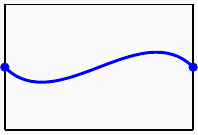
\includegraphics[scale=0.1]{Images/hcross.png}}}\right)$ e $\VC(n, m) \colonequals \{\exists$ cruzamento vertical em $\text{R}(n, m)\}$ $\left(\visible<6>{\raisebox{-.31\height}{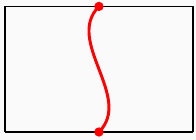
\includegraphics[scale=0.1]{Images/vcross.png}}}\right)$. % Aqui, eu usei o arquivo hcross.tex para gerar o rascunho da imagem
		\end{myitemize}
	\end{frame}

	\begin{frame}[t]
	\frametitle{Aplicações em percolação Bernoulli ($\LX^d$)}
		Notações e definições:
		\vspace{2.6pt}
		\begin{myitemize}
			\item Defina um \textit{reticulado dual} $(\LX^2)^{\star} = ((\ZX^2)^{\star}, (\text{E}^2)^{\star})$ onde $(\ZX^2)^{\star} = \ZX^2 + \left(\frac{1}{2}, \frac{1}{2}\right)$ é conjunto de vértices e $(\text{E}^2)^{\star} = \{(x^{\star}, y^{\star}) \in (\ZX^2)^{\star} \times (\ZX^2)^{\star} : \delta(x^{\star}, y^{\star}) = 1\}$ é conjunto de elos. Além disso, para cada elo $e \in \text{E}^2$, denote por $e^{\star} \in (\text{E}^2)^{\star}$ o elo no \textit{reticulado dual} que o cruza; por fim, defina $\omega^{\star}_{e^{\star}} \colonequals 1 - \omega_e$.
		\end{myitemize}
		\begin{figure}
			\begin{tikzpicture}[scale = 1]
	\node[black] at (-0.20, -0.20) {{\footnotesize $0^{\phantom{\star}}$}};
	\draw[solid, black] (-3, -2) -- (3, -2);
	\draw[solid, black] (-3, -1) -- (3, -1);
	\draw[solid, black] (-3,  0) -- (3,  0);
	\draw[solid, black] (-3,  1) -- (3,  1);
	\draw[solid, black] (-3,  2) -- (3,  2);
	\draw[solid, black] (-2, -3) -- (-2, 3);
	\draw[solid, black] (-1, -3) -- (-1, 3);
	\draw[solid, black] (0,  -3) -- (0,  3);
	\draw[solid, black] (1,  -3) -- (1,  3);
	\draw[solid, black] (2,  -3) -- (2,  3);
	\draw[black] (-2, -2) circle (2pt);
	\draw[black] (-2, -1) circle (2pt);
	\draw[black] (-2,  0) circle (2pt);
	\draw[black] (-2,  1) circle (2pt);
	\draw[black] (-2,  2) circle (2pt);
	\draw[black] (-1, -2) circle (2pt);
	\draw[black] (-1, -1) circle (2pt);
	\draw[black] (-1,  0) circle (2pt);
	\draw[black] (-1,  1) circle (2pt);
	\draw[black] (-1,  2) circle (2pt);
	\draw[black] (0,  -2) circle (2pt);
	\draw[black] (0,  -1) circle (2pt);
	\draw[black] (0,   0) circle (2pt);
	\draw[black] (0,   1) circle (2pt);
	\draw[black] (0,   2) circle (2pt);
	\draw[black] (1,  -2) circle (2pt);
	\draw[black] (1,  -1) circle (2pt);
	\draw[black] (1,   0) circle (2pt);
	\draw[black] (1,   1) circle (2pt);
	\draw[black] (1,   2) circle (2pt);
	\draw[black] (2,  -2) circle (2pt);
	\draw[black] (2,  -1) circle (2pt);
	\draw[black] (2,   0) circle (2pt);
	\draw[black] (2,   1) circle (2pt);
	\draw[black] (2,   2) circle (2pt);
	
	\node[blue] at (0.30, 0.30) {{\footnotesize $0^{\star}$}};
	\draw[densely dashed, blue] (-2.5, -1.5) -- (3.5, -1.5);
	\draw[densely dashed, blue] (-2.5, -0.5) -- (3.5, -0.5);
	\draw[densely dashed, blue] (-2.5,  0.5) -- (3.5,  0.5);
	\draw[densely dashed, blue] (-2.5,  1.5) -- (3.5,  1.5);
	\draw[densely dashed, blue] (-2.5,  2.5) -- (3.5,  2.5);
	\draw[densely dashed, blue] (-1.5, -2.5) -- (-1.5, 3.5);
	\draw[densely dashed, blue] (-0.5, -2.5) -- (-0.5, 3.5);
	\draw[densely dashed, blue] (0.5,  -2.5) -- (0.5,  3.5);
	\draw[densely dashed, blue] (1.5,  -2.5) -- (1.5,  3.5);
	\draw[densely dashed, blue] (2.5,  -2.5) -- (2.5,  3.5);
	\draw[blue] (-1.5, -1.5) circle (2pt);
	\draw[blue] (-1.5, -0.5) circle (2pt);
	\draw[blue] (-1.5,  0.5) circle (2pt);
	\draw[blue] (-1.5,  1.5) circle (2pt);
	\draw[blue] (-1.5,  2.5) circle (2pt);
	\draw[blue] (-0.5, -1.5) circle (2pt);
	\draw[blue] (-0.5,  0.5) circle (2pt);
	\draw[blue] (-0.5, -0.5) circle (2pt);
	\draw[blue] (-0.5,  1.5) circle (2pt);
	\draw[blue] (-0.5,  2.5) circle (2pt);
	\draw[blue] (0.5,  -1.5) circle (2pt);
	\draw[blue] (0.5,  -0.5) circle (2pt);
	\draw[blue] (0.5,   0.5) circle (2pt);
	\draw[blue] (0.5,   1.5) circle (2pt);
	\draw[blue] (0.5,   2.5) circle (2pt);
	\draw[blue] (1.5,  -1.5) circle (2pt);
	\draw[blue] (1.5,  -0.5) circle (2pt);
	\draw[blue] (1.5,   0.5) circle (2pt);
	\draw[blue] (1.5,   1.5) circle (2pt);
	\draw[blue] (1.5,   2.5) circle (2pt);
	\draw[blue] (2.5,  -1.5) circle (2pt);
	\draw[blue] (2.5,  -0.5) circle (2pt);
	\draw[blue] (2.5,   0.5) circle (2pt);
	\draw[blue] (2.5,   1.5) circle (2pt);
	\draw[blue] (2.5,   2.5) circle (2pt);	
\end{tikzpicture}
			\vspace{-3pt}
			\caption{\justifying Reticulado original $\LX^2$ (linha sólida) e \textit{reticulado dual} $(\LX^2)^{\star}$ (linha tracejada).}
			\label{fig:caixas-iteradas}
		\end{figure}
	\end{frame}
	
	\subsection{Ponto crítico para percolação em $\LX^2$}
	\begin{frame}[t]
		\frametitle{Ponto crítico para percolação em $\LX^2$}
		\begin{mythm}[Kesten, 1980] \label{thm:kesten}
			O ponto crítico para percolação Bernoulli em $\LX^2$ é $\frac{1}{2}$.
		\end{mythm}
		\vspace{-3pt}
		O Teorema \ref{thm:kesten} será demonstrado em duas partes. Primeiro, veremos o resultado de que $p_c(2) \geq \frac{1}{2}$ e, por fim, provaremos que $p_c(2) \leq \frac{1}{2}$. \pause
		\begin{mypro}\label{prop:pc-maior-meio}
			Existe $\alpha > 0$ tal que, para todo $n \geq 1$, $\PX_{\frac{1}{2}}(0 \leftrightarrow \partial \Lambda_n) \leq n^{-\alpha}$. Em particular $p_c \geq \frac{1}{2}$.
		\end{mypro}
		\vspace{-3pt}
		A partir da Proposição \ref{prop:pc-maior-meio} e recordando a definição de $p_c(d)$, para verificar que $p_c(2) \geq \frac{1}{2}$, basta notar que, se $n \to +\infty$, então $\PX_{\frac{1}{2}}(\{\omega \in \Omega : |C_0(\omega)| = +\infty\}) = 0$. \pause
		\begin{mypro}\label{prop:beta}
			Para qualquer $p > \frac{1}{2}$, existe $\beta = \beta(p) > 0$, tal que 
			\begin{align*}
			\PX_p(\HL(2n, n)) \geq 1 - \frac{1}{\beta}n^{-\beta}.
			\end{align*}
		\end{mypro}
	\end{frame}

	\begin{frame}[t]
		\frametitle{Ponto crítico para percolação em $\LX^2$}
		\texttt{Demonstração:}
		
		Comece por definir a função Booleana $f_n(\omega) \colonequals \IX_{\HL(2n, n)}(\omega)$. Fixe um elo $e$ em $\text{R}(2n, n)$ e veja que se $\diffe \neq 0$, então existe um caminho aberto na rede dual que conecta a parte de cima (de baixo, respec.) de uma caixa do tipo $\text{R}^{\star} = \left[\frac{1}{2}, 2n - \frac{1}{2}\right] \times [-\frac{1}{2}, n + \frac{1}{2}]$ à extremidade superior (inferior, respec.) do elo $e^{\star}$. Nesse caso, note que pelo menos um dos dois ``braços'' de elos abertos na rede dual com início em $e^{\star}$ tem tamanho $ \geq \frac{n}{2}$.
		\vspace{-12pt}
		\begin{figure}
			\begin{tikzpicture}[scale = 0.55]

	\draw[solid, black] (0, 0) -- (8, 0);
	\draw[solid, black] (0, 4) -- (8, 4);
	\draw[solid, black] (0, 0) -- (0, 4);
	\draw[solid, black] (8, 0) -- (8, 4);
	
	\draw[solid, very thick, black] (3.75, 2) -- (4.25, 2);
	\node[black] at (3.65, 1.75) {{\small $e$}};
	\draw[solid, very thick, black] (4, 1.75) -- (4, 2.25);
	\node[black] at (4.35, 2.40) {{\small $e^{\star}$}};
	
	
	\draw[dashed, black] (0.25, -0.25) -- (7.75, -0.25);
	\draw[dashed, black] (0.25, 4.25) -- (7.75, 4.25);
	\draw[dashed, black] (0.25, -0.25) -- (0.25, 4.25);
	\draw[dashed, black] (7.75, -0.25) -- (7.75, 4.25);
	
	\draw[solid, thick, black] (0, 2) to[out = -45, in = 135] (3.75, 2);
	\draw[solid, thick, black] (4.25, 2) to[out = -45, in = 135] (8, 2);
	\draw[fill] (3.75, 2) circle (2pt);
	\draw[fill] (4.25, 2) circle (2pt);
	\draw[fill] (0, 2) circle (2pt);
	\draw[fill] (8, 2) circle (2pt);
	
	\draw[dashed, thick, black] (4, -0.25) to[out = 45, in = -135] (4, 1.75);
	\draw[dashed, thick, black] (4,  2.25) to[out = 45, in = -135] (4, 4.25);
	\draw[draw] (4, 1.75) circle (2pt);
	\draw[draw] (4, 2.25) circle (2pt);
	\draw[draw] (4, -0.25) circle (2pt);
	\draw[draw] (4,  4.25) circle (2pt);
	
	\draw [decorate, decoration = {brace, amplitude = 12pt, mirror}, xshift = 0pt, yshift = -8pt] (0, 0) -- (8, 0) node [black, midway, xshift = 0pt, yshift = -18pt] {\small $2n$};
	
	\draw [decorate, decoration = {brace, amplitude = 6pt, mirror}, xshift = 4pt, yshift = 0pt] (8, 0) -- (8, 4) node [black, midway, xshift = 12pt, yshift = 0pt] {\small $n$};
	
	\node[black] at (-0.25, 0.15) {{\small $\text{R}^{\phantom{\star}}$}};
	\node[black] at (0.45, 4.55) {{\small $\text{R}^{\star}$}};
	
\end{tikzpicture}
			\vspace{-9pt}
			\caption{\justifying Caixas $\text{R} = \text{R}(2n, n)$ e $\text{R}^{\star}$ para um elo fixado $e$, tal que $\nabla_e f_n(\omega) \neq 0$.}
			\label{fig:caixa-2n}
		\end{figure}
		
	\end{frame}

	\begin{frame}[t]
		\frametitle{Ponto crítico para percolação em $\LX^2$}
		Como os estados dos elos de $\omega^{\star}$ são determinados, de maneira independente, seguindo uma distribuição Bernoulli de parâmetro $1 - p$, a Proposição \ref{prop:pc-maior-meio} nos dá que, para $p > \frac{1}{2}$, 
		\begin{align*}
		\text{Inf}_e(f_n(\omega)) = \PX_p(f_n(\omega) \neq f_n(\flipe)) &\leq 2\PX_{1-p}\left(0 \leftrightarrow \partial\Lambda_{\frac{n}{2}}\right), \text{ por inclus. de eventos} \\
		&\leq 2\PX_{\frac{1}{2}}\left(0 \leftrightarrow \partial\Lambda_{\frac{n}{2}}\right), \text{ já que $1 - p < \frac{1}{2}$} \\
		&\leq \frac{1}{N}, \text{ onde $N = \frac{1}{2}\left(\frac{n}{2}\right)^{\alpha}$}.
		\end{align*}\pause
		O que acabamos de ver é que, para todo $e \in \text{R}(2n ,n)$, $\text{Inf}_e(f_n(\omega)) \leq \frac{1}{N}$; o que, pelo Teorema \ref{thm:talagrand}, implica em dizer que, para $p > \frac{1}{2}$,
		\begin{align}\label{eq:thm-grupo}
		F_n^{\prime}(p) \geq c^{\prime}\,\ln(N)\,\VX_p(f_n(\omega)), \text{ onde } c^{\prime} = \left(c\,\ln\frac{1}{p(1-p)}\right)^{-1}.
		\end{align}
		
		Assim, integrando a Expressão \ref{eq:thm-grupo} entre $\frac{1}{2}$ e $p$, obtemos
		\begin{align*}
		F_n(p) \geq 1 - \frac{1}{F_n\left(\frac{1}{2}\right)} \, N^{-c^{\prime}\,\left(p - \frac{1}{2}\right)} \geq 1 - \frac{1}{\beta} n^{-\beta},
		\end{align*}
		para $\beta$ pequeno o suficiente.\hspace{\fill}\qed
	\end{frame}

	\begin{frame}[t]
		\frametitle{Ponto crítico para percolação em $\LX^2$}
		\texttt{Demonstração (Teorema \ref{thm:kesten}):}
			
		Para provar que, em $d = 2$, $p_c(d)$ é igual a $\frac{1}{2}$, basta mostrar que $p_c(2) \leq \frac{1}{2}$; já que, pela Proposição \ref{prop:pc-maior-meio}, temos que $p_c(2) \geq \frac{1}{2}$. Porém, a estratégia utilizada aqui será a de mostrar que, para $p > \frac{1}{2}$, existe, com probabilidade $1$, aglomerado de tamanho \hspace{1pt}infinito.\pause
		
		Defina, como na Figura \ref{fig:caixas-iteradas}, os eventos $A_n \colonequals \HL(2^{n+1}, 2^n)$ e $B_n \colonequals \VL(2^n, 2^{n+1})$.
		
		\begin{figure}
			\begin{tikzpicture}[scale = 0.75]

	\draw[solid, black] (0, 0) -- (2, 0);
	\draw[solid, black] (2, 0) -- (2, 1);
	\draw[solid, black] (2, 1) -- (0, 1);
	\draw[solid, black] (0, 1) -- (0, 0);
	
	\draw[solid, black] (0, 0) -- (2, 0);
	\draw[solid, black] (2, 0) -- (2, 4);
	\draw[solid, black] (2, 4) -- (0, 4);
	\draw[solid, black] (0, 4) -- (0, 0);

	\draw[solid, black] (0, 0) -- (8, 0);
	\draw[solid, black] (8, 0) -- (8, 4);
	\draw[solid, black] (8, 4) -- (0, 4);
	\draw[solid, black] (0, 4) -- (0, 0);
	
	\draw[solid, thick, black] (0, 0.5) to[out = 45, in = -135] (2, 0.5);
	\draw[solid, thick, black] (1.0, 0) to[out = 45, in = -135] (1.0, 4);
	\draw[solid, thick, black] (0, 2.0) to[out = 45, in = -135] (8, 2.0);
	
	\draw[fill] (0, 0.5) circle (2pt);
	\draw[fill] (2, 0.5) circle (2pt);
	\draw[fill] (1,   0) circle (2pt);
	\draw[fill] (1,   4) circle (2pt);
	\draw[fill] (0,   2) circle (2pt);
	\draw[fill] (8,   2) circle (2pt);
	
	\draw[black] (0, 0) circle (2pt);
	\node[black] at (-0.5, -0.25) {{\footnotesize $(0, 0)$}};
	
	\draw [decorate, decoration = {brace, amplitude = 6pt, mirror}, xshift = 0pt, yshift = -2pt] (0, 0) -- (2, 0) node [black, midway, xshift = 0pt, yshift = -12pt] {\footnotesize $2$};
	
	\draw [decorate, decoration = {brace, amplitude = 6pt, mirror}, xshift = 0pt, yshift = -18pt] (0, 0) -- (8, 0) node [black, midway, xshift = 0pt, yshift = -12pt] {\footnotesize $8$};

	\draw [decorate, decoration = {brace, amplitude = 6pt}, xshift = -2pt, yshift = 0pt] (0, 0) -- (0, 1) node [black, midway, xshift = -12pt, yshift = 0pt] {\footnotesize $1$};

	\draw [decorate, decoration = {brace, amplitude = 6pt}, xshift = -18pt, yshift = 0pt] (0, 0) -- (0, 4) node [black, midway, xshift = -12pt, yshift = 0pt] {\footnotesize $4$};

%	
%	\draw[solid, black] (-4, -4) -- ( 4, -4);
%	\draw[solid, black] ( 4, -4) -- ( 4,  4);
%	\draw[solid, black] ( 4,  4) -- (-4,  4);
%	\draw[solid, black] (-4,  4) -- (-4, -4);
%	
%	\draw[dashed, black] (-2, -4) -- (-2, 4);
%	\draw[dashed, black] ( 2, -4) -- ( 2, 4);
%	\draw[dashed, black] (-4, -2) -- ( 4,-2);
%	\draw[dashed, black] (-4,  2) -- ( 4, 2);
%	
%	\draw[black] ( 0,  0) circle (3.35pt);
%	\node[black] at (0, -.5) {{\footnotesize $(0, 0)$}};
%	\node[black] at (-2.4, -1.65) {{\small $\Lambda_{k\phantom{2}}$}};
%	\node[black] at (-4.6, -3.65) {{\small $\Lambda_{2k}$}};
%	
%	\draw[fill] ( -1,  1) circle (3.35pt);
%	\draw[fill] ( -4,  1) circle (3.35pt);
%	
%	\draw[solid, thick, black] (-1, 1) to[out = 135, in = -45] (-4, 1);
%	
%	\draw [decorate, decoration = {brace, amplitude = 6pt, mirror}, xshift = 4pt, yshift = 0pt] (2, -2) -- (2, 2) node [black, midway, xshift = 14pt, yshift = 0pt] {\small $2k$};
%	
%	\draw [decorate, decoration = {brace, amplitude = 6pt, mirror}, xshift = 4pt, yshift = 0pt] (4, -4) -- (4, 4) node [black, midway, xshift = 14pt, yshift = 0pt] {\small $4k$};
	
\end{tikzpicture}
			\vspace{-9pt}
			\caption{\justifying Ocorrência (alternada) dos eventos $\HL(2^{n+1}, 2^n)$ e $\VL(2^n, 2^{n+1})$ para $n \in \{0, 1, 2\}$.}
			\label{fig:caixas-iteradas}
		\end{figure}
	\end{frame}

	\begin{frame}[t]
	\frametitle{Ponto crítico para percolação em $\LX^2$}
		Agora, note que se $A_n$ e $B_n$ ocorrem para todo $n \in \NX$, com exceção de uma quantidade finita de vezes, então existe aglomerado de tamanho infinito em $\omega$.
		
		Assim, pela Proposição \ref{prop:beta}, e considerando um retângulo do tipo $\text{R}(2^{n+1}, 2^n)$, temos que, para $p > \frac{1}{2}$,
		\begin{align}\label{eq:ineq-borel}
		\sum_{n = 1}^{+\infty}\PX_p({A_n}^c) \leq \frac{1}{\beta} \sum_{n = 1}^{+\infty} 2^{-\beta\,n}.
		\end{align}\pause	
		Da Expressão \ref{eq:ineq-borel}, perceba que $\sum_{n=1}^{+\infty}2^{-\beta\,n}$ converge; logo, por Borel-Cantelli, $\PX({A_n}^c$ infinitas vezes$) = 0$. O que significa que, com probabilidade $1$, $A_n$ não ocorre, no máximo, uma quantidade finitas de vezes. Usando invariância por translação, $\PX_p({B_n}^c \text{ infinitas vezes}) = 0$. Dessa forma, como $A_n$ e $B_n$ ocorrem para todo $n \in \NX$, exceto para uma quantidade finita de termos dessas sequências, então existe, com probabilidade $1$, aglomerado de tamanho infinito em $\omega$.\hspace{\fill}\qed
	\end{frame}

	\begin{frame}[t]
	\frametitle{Ponto crítico para percolação em $\LX^2$}
		Alternativamente, podemos adotar a seguinte estratégia. Veja que, para $p = \frac{1}{2}$, e relembrando da definição da rede dual; i.e., se $\omega \sim \PX_p$, então $\omega^{\star} \sim \PX_{1-p}$,
		\begin{align*}
			\PX_{\frac{1}{2}}(\HL(n + 1, n)) &= 1 - \PX_{\frac{1}{2}}(\HL(n + 1, n)^c) = 1 - \PX_{\frac{1}{2}}\left(\VL^{\star}\left(\left[\frac{1}{2}, n + \frac{1}{2}\right]\times\left[-\frac{1}{2}, n + \frac{1}{2}\right]\right)\right) \\
			&= 1 - \PX_{\frac{1}{2}}(\HL(n + 1, n)) \implies \PX_{\frac{1}{2}}(\HL(n + 1, n)) = \frac{1}{2}, ~\forall n \in \NX.
		\end{align*} \pause
		Assim, se pudermos mostrar que, para $p \in (p_c, 1]$, $\PX_p(\HL(n + 1, n)) \to 1$, quando $n \to +\infty$, então temos que $p_c \geq \frac{1}{2}$. \pause
		
		Agora, devemos mostrar que $p_c \leq \frac{1}{2}$. Para isso, suponha $p_c > \frac{1}{2}$. Assim,
		\begin{align*}
			\PX_{\frac{1}{2}}(\HL(n + 1, n)) \leq \PX_{\frac{1}{2}}\left(\bigcup_{i = 1}^{n} (0 \leftrightarrow \partial\Lambda_n)\right) \leq n \, \PX_{\frac{1}{2}}(0 \leftrightarrow \partial\Lambda_n);
		\end{align*}
		o que, se, para $p \in [0, p_c)$, pudermos mostrar que $\PX_p(0 \leftrightarrow \partial\Lambda_n) \to 0$ ``rápido o suficiente'', quando $n \to +\infty$, é um absurdo $-$ já que $\PX_{\frac{1}{2}}(\HL(n + 1, n)) = \frac{1}{2}$, $\forall n \in \NX$.
		
		Assim, queremos provar que, para $p \in [0, p_c)$, $\PX_p(0 \leftrightarrow \partial\Lambda_n)$ decai (exponencialmente rápido) com $n$.
	\end{frame}

	\subsection{\textit{Sharpness} da transição de fase para percolação Bernoulli em $\LX^d$}
	\begin{frame}[t]
		\frametitle{\textit{Sharpness} da transição de fase para percolação Bernoulli em $\LX^d$}
		\begin{mythm}[H. Duminil-Copin, A. Raoufi e V. Tassion, 2019]\label{thm:decai-exp}
			Para percolação Bernoulli em $\ZX^d$,
			\begin{enumerate}
				\item Para $p < p_c$, existe $c_p > 0$ tal que, para todo $n \geq 1$, $\PX_p(0 \leftrightarrow \partial\Lambda_n) \leq e^{-c_p \, n}$.
				\item (Mean Field Lower Bound) Existe $c > 0$ tal que $p > p_c$, $\PX_p(0 \leftrightarrow +\infty) \geq c\,(p - p_c)$.
			\end{enumerate}
		\end{mythm}
		\vspace{-3pt}
		Outras provas para resultados como o do Teorema \ref{thm:decai-exp} foram desenvolvidas por Menshikov (1986) e Aizenman e Barsky (1987), além de H. Duminil-Copin e V. Tassion (2016).\pause
		\begin{mylem}\label{lem:analise}
			Considere uma sequência de funções convergentes $f_n: [0, \bar{x}] \to [0, M]$ diferenciáveis e crescentes em $x$ tal que, para todo $n \geq 1$,
			\vspace{-3pt}
			\begin{align*}
			f_n^{\prime} \geq \frac{n}{\Sigma_n} \, f_n,
			\end{align*}\vspace{-6pt}
			onde $\Sigma_n = \sum_{k = 0}^{n - 1}f_k$. Então existe $\tilde{x} \in [0, \bar{x}]$ tal que
			\begin{enumerate}[a.]
				\item Para qualquer $x < \tilde{x}$, existe $c_x > 0$ tal que, para qualquer $n \geq 1$, $f_n(x) \leq e^{-c_x\,n}$.
				\item Para qualquer $x > \tilde{x}$, $f = \lim_{n \to +\infty} f_n$ satisfaz $f(x) \geq x - \bar{x}$.
			\end{enumerate}
		\end{mylem}
	\end{frame}

	\begin{frame}[t]
		\frametitle{\textit{Sharpness} da transição de fase para percolação Bernoulli em $\LX^d$}
		Defina $\theta_n(p) \colonequals \PX_p(0 \leftrightarrow \partial\Lambda_n)$ e $S_n \colonequals \sum_{s = 0}^{n-1}\theta_s(p)$. Nesse caso, vale o resultado abaixo.
		\begin{mypro}\label{prop:decai-exp}
			Para qualquer $n \geq 1$, temos que
			\begin{align*}
			\sum_{e \in \text{E}_n} \text{Inf}_e(\IX_{0\leftrightarrow\partial\Lambda_n}(\omega)) \geq \frac{n}{S_n} \, \theta_n(p) \, (1 - \theta_n(p)),
			\end{align*}
			onde $\text{E}_n$ é o conjunto de elos tal que as duas extremidades de $e$ estão em $\Lambda_n$.
		\end{mypro}
		\vspace{-3pt}
%		\begin{minipage}[t]{0.55 \textwidth}
%			Para a demonstração da Proposição \ref{prop:decai-exp}, é suficiente provar que para qualquer $1 \leq s \leq n$, temos um algoritmo \textbf{T} para $\IX_{0\leftrightarrow\partial\Lambda_n}(\omega)$ tal que, para todo $e = (x, y) \in \text{E}_n$,
%			\begin{align*}
%			\delta_e(\text{\textbf{T}}) \leq \PX_p(x \leftrightarrow \partial\Lambda_s) + \PX_p(y \leftrightarrow \partial\Lambda_s).
%			\end{align*}
%		\end{minipage}\pause
%		\begin{minipage}[t]{0.45 \textwidth}
%			\begin{figure}
%				\begin{tikzpicture}[scale = 1]

	\begin{scope}	
		\clip (0.60, 0) to[out = 86, in = 135] (1.25, 0.75) to[out = -45, in = 135] (1.75, -0.5) to[out = -45, in = -95] (0.60, 0); % Área limitada
		\draw[pattern = north east lines, pattern color = black!30] (-2 , -2) rectangle (2, 2); % Área total
	\end{scope}

	\draw[solid, black] (-2,  2) -- ( 2,  2);
	\draw[solid, black] ( 2,  2) -- ( 2, -2);
	\draw[solid, black] ( 2, -2) -- (-2, -2);
	\draw[solid, black] (-2, -2) -- (-2,  2);
	
	\draw[dashed, black] (-1,  1) -- ( 1,  1);
	\draw[dashed, black] ( 1,  1) -- ( 1, -1);
	\draw[dashed, black] ( 1, -1) -- (-1, -1);
	\draw[dashed, black] (-1, -1) -- (-1,  1);
	
	\draw[black] ( 0,  0) circle (1.25pt);
	\node[black] at (0, -.35) {{\footnotesize $0$}};
	\node[black] at (1.80, -2.30) {{\small $\Lambda_n$}};
	\node[black] at (0.80, -1.30) {{\small $\Lambda_s$}};
%	\node[red] at (1.25,  1.25) {{\tiny $C_{\partial\Lambda_k}(\omega)$}};
	
	\draw[solid, black] (0.60, 0) to[out = 86, in = 135] (1.25, 0.75) to[out = -45, in = 135] (1.75, -0.5) to[out = -45, in = -95] (0.60, 0);


%	\draw[solid, thick, black] (0, 2) to[out = -45, in = 135] (3.75, 2);
%	\draw[solid, thick, black] (4.25, 2) to[out = -45, in = 135] (8, 2);
%	\draw[fill] (3.75, 2) circle (2pt);
%	\draw[fill] (4.25, 2) circle (2pt);
%	\draw[fill] (0, 2) circle (2pt);
%	\draw[fill] (8, 2) circle (2pt);
%	
%	\draw[dashed, thick, black] (4, -0.25) to[out = 45, in = -135] (4, 1.75);
%	\draw[dashed, thick, black] (4,  2.25) to[out = 45, in = -135] (4, 4.25);
%	\draw[draw] (4, 1.75) circle (2pt);
%	\draw[draw] (4, 2.25) circle (2pt);
%	\draw[draw] (4, -0.25) circle (2pt);
%	\draw[draw] (4,  4.25) circle (2pt);
%	
%	\draw [decorate, decoration = {brace, amplitude = 12pt, mirror}, xshift = 0pt, yshift = -8pt] (0, 0) -- (8, 0) node [black, midway, xshift = 0pt, yshift = -18pt] {\small $2n$};
%	
%	\draw [decorate, decoration = {brace, amplitude = 6pt, mirror}, xshift = 4pt, yshift = 0pt] (8, 0) -- (8, 4) node [black, midway, xshift = 12pt, yshift = 0pt] {\small $n$};
%	
%	\node[black] at (-0.25, 0.15) {{\small $\text{R}^{\phantom{\star}}$}};
%	\node[black] at (0.45, 4.55) {{\small $\text{R}^{\star}$}};
	
\end{tikzpicture}
%				\vspace{-9pt}
%				\caption{\justifying Algoritmo \text{\textbf{T}} para $\IX_{0\leftrightarrow\partial\Lambda_n}(\omega)$.}
%				\label{fig:caixa-k}
%			\end{figure}
%		\end{minipage}
			Para a demonstração da Proposição \ref{prop:decai-exp}, é suficiente provar que para qualquer $1 \leq s \leq n$, temos um algoritmo \textbf{T} para $\IX_{0\leftrightarrow\partial\Lambda_n}(\omega)$ tal que, para todo $e = (x, y) \in \text{E}_n$,
			\begin{align*}
				\delta_e(\text{\textbf{T}}) \leq \PX_p(x \leftrightarrow \partial\Lambda_s) + \PX_p(y \leftrightarrow \partial\Lambda_s).
			\end{align*} \pause
			De fato, pelo Teorema \ref{thm:osss} (Desigualdade de OSSS), 
			\begin{align*}
			\sum_{s = 1}^n\VX_p(\IX_{0 \leftrightarrow \partial\Lambda_n}(\omega)) \leq \sum_{s = 1}^n p\,(1-p) \sum_{e \in \text{E}_n}(\PX_p(x \leftrightarrow \partial\Lambda_s) + \PX_p(y \leftrightarrow \partial\Lambda_s)) \, \text{Inf}_e(\IX_{0 \leftrightarrow \partial\Lambda_n}(\omega)).
			\end{align*}
			Reescrevendo $\VX_p(\IX_{0 \leftrightarrow \partial\Lambda_n}(\omega))$ e dizendo que $\sum_{s = 1}^n \PX_p(x \leftrightarrow \partial\Lambda_s) + \PX_p(y \leftrightarrow \partial\Lambda_s) \leq 4\, S_n$, temos o resultado desejado.
	\end{frame}

	\begin{frame}[t]
	\frametitle{\textit{Sharpness} da transição de fase para percolação Bernoulli em $\LX^d$}
		Nesse caso, o algoritmo de exploração \textbf{T} poderá se representado, para cada $1 \leq s \leq n$, pela Figura \ref{fig:caixa-s}.
		\vspace{6pt}
		\begin{figure}
			\begin{tikzpicture}[scale = 1]

	\begin{scope}	
		\clip (0.60, 0) to[out = 86, in = 135] (1.25, 0.75) to[out = -45, in = 135] (1.75, -0.5) to[out = -45, in = -95] (0.60, 0); % Área limitada
		\draw[pattern = north east lines, pattern color = black!30] (-2 , -2) rectangle (2, 2); % Área total
	\end{scope}

	\draw[solid, black] (-2,  2) -- ( 2,  2);
	\draw[solid, black] ( 2,  2) -- ( 2, -2);
	\draw[solid, black] ( 2, -2) -- (-2, -2);
	\draw[solid, black] (-2, -2) -- (-2,  2);
	
	\draw[dashed, black] (-1,  1) -- ( 1,  1);
	\draw[dashed, black] ( 1,  1) -- ( 1, -1);
	\draw[dashed, black] ( 1, -1) -- (-1, -1);
	\draw[dashed, black] (-1, -1) -- (-1,  1);
	
	\draw[black] ( 0,  0) circle (1.25pt);
	\node[black] at (0, -.35) {{\footnotesize $0$}};
	\node[black] at (1.80, -2.30) {{\small $\Lambda_n$}};
	\node[black] at (0.80, -1.30) {{\small $\Lambda_s$}};
%	\node[red] at (1.25,  1.25) {{\tiny $C_{\partial\Lambda_k}(\omega)$}};
	
	\draw[solid, black] (0.60, 0) to[out = 86, in = 135] (1.25, 0.75) to[out = -45, in = 135] (1.75, -0.5) to[out = -45, in = -95] (0.60, 0);


%	\draw[solid, thick, black] (0, 2) to[out = -45, in = 135] (3.75, 2);
%	\draw[solid, thick, black] (4.25, 2) to[out = -45, in = 135] (8, 2);
%	\draw[fill] (3.75, 2) circle (2pt);
%	\draw[fill] (4.25, 2) circle (2pt);
%	\draw[fill] (0, 2) circle (2pt);
%	\draw[fill] (8, 2) circle (2pt);
%	
%	\draw[dashed, thick, black] (4, -0.25) to[out = 45, in = -135] (4, 1.75);
%	\draw[dashed, thick, black] (4,  2.25) to[out = 45, in = -135] (4, 4.25);
%	\draw[draw] (4, 1.75) circle (2pt);
%	\draw[draw] (4, 2.25) circle (2pt);
%	\draw[draw] (4, -0.25) circle (2pt);
%	\draw[draw] (4,  4.25) circle (2pt);
%	
%	\draw [decorate, decoration = {brace, amplitude = 12pt, mirror}, xshift = 0pt, yshift = -8pt] (0, 0) -- (8, 0) node [black, midway, xshift = 0pt, yshift = -18pt] {\small $2n$};
%	
%	\draw [decorate, decoration = {brace, amplitude = 6pt, mirror}, xshift = 4pt, yshift = 0pt] (8, 0) -- (8, 4) node [black, midway, xshift = 12pt, yshift = 0pt] {\small $n$};
%	
%	\node[black] at (-0.25, 0.15) {{\small $\text{R}^{\phantom{\star}}$}};
%	\node[black] at (0.45, 4.55) {{\small $\text{R}^{\star}$}};
	
\end{tikzpicture}
			\vspace{-6pt}
			\caption{\justifying Algoritmo de exploração \text{\textbf{T}}, com $1 \leq s \leq n$, para a função $\IX_{0\leftrightarrow\partial\Lambda_n}(\omega)$.}
			\label{fig:caixa-s}
		\end{figure}
		
		\vspace{-6pt}
		Aqui, lembre-se de que queremos demonstrar que $\delta_e(\text{\textbf{T}}) \leq \PX_p(x \leftrightarrow \partial\Lambda_s) + \PX_p(y \leftrightarrow \partial\Lambda_s)$.
	\end{frame}

	\begin{frame}[t]
		\frametitle{\textit{Sharpness} da transição de fase para percolação Bernoulli em $\LX^d$}
		\texttt{Demonstração:}
		
		Defina o conjunto de índices $\mathbf{e}$ utilizando duas sequências $\partial\Lambda_s = \text{V}_0 \subset \text{V}_1 \subset \cdots \subset \text{V}_n$ e $\emptyset = \text{E}_0 \subset \text{E}_1 \subset \cdots \subset \text{E}_n$. Aqui, $\text{V}_t$ representa o conjunto de vértices que o algoritmo verificou estar conectado a $\partial\Lambda_s$ e $\text{E}_t$ representa o conjunto de elos explorados pelo algoritmo até o instante $t$.\pause
		
		Fixando uma ordem para os elos de $\text{E}_n$, defina $\text{V}_0 = \partial\Lambda_s$ e $\text{E}_0 = \emptyset$. Assuma, então, que os conjuntos $\text{V}_t \subset \text{V}_n$ e $\text{E}_t \subset \text{E}_n$ foram construídos de tal forma que, em $t$, uma das duas situações a segui se aplica:
		
		\begin{enumerate}[a.]
			\item Se existe elo $e = (x, y)$ em $\text{E}_n \text{~\textbackslash~} \text{E}_t$ tal que $x \in \text{V}_t$ e $y \not\in \text{V}_t$ (se existir mais de um, escolha o menor deles $-$ de acordo com a ordem estabelecida), então defina $\mathbf{e}_{t+1} \colonequals e$, $\text{E}_{t + 1} \colonequals \text{E}_t \cup \{e\}$ e
			\[ \text{V}_{t + 1} \colonequals
			\begin{cases}
			\text{V}_t \cup \{y\} &\text{ se } \omega_e = 1 \\
			\text{V}_t &\text{ caso contrário}.
			\end{cases}
			\]
			\item Se $e$ não existe, então defina $\mathbf{e}_{t+1}$ como o menor elo em $\text{E}_n \text{~\textbackslash~} \text{E}_t$ (de acordo com a ordem estabelecida), $\text{E}_{t + 1} \colonequals \text{E}_t \cup \{e\}$ e $\text{V}_{t + 1} \colonequals \text{V}_t$.
		\end{enumerate}
	\end{frame}

	\begin{frame}[t]
	\frametitle{\textit{Sharpness} da transição de fase para percolação Bernoulli em $\LX^d$}
		Perceba que, enquanto estivermos na situação ``a$.$'', ainda estamos descobrindo elos que fazem parte da componente conectada a $\partial\Lambda_s$; ao passo que, assim que mudamos para a situação ``b$.$'', nós permanecemos nela. Nesse caso, $\tau(\omega)$ não é maior que o último $t$ para o qual ainda estamos na situação ``a$.$''.
		
		\par Relembrando a definição de $\delta_e(\text{\textbf{T}}) \colonequals \PX_p(\exists t \leq \tau(\omega) : e_t = e)$, temos que
		\begin{align*}
		\PX_p(\exists t \leq \tau(\omega) : e_t = e) &\leq \PX_p\left(\{x \leftrightarrow \partial\Lambda_s\} \cup \{y \leftrightarrow \partial\Lambda_s\}\right) \\
		&\leq \PX_p(x \leftrightarrow \partial\Lambda_s) + \PX_p(y \leftrightarrow \partial\Lambda_s),
		\end{align*}
		finalizando a demonstração.\hspace{\fill}\qed
	\end{frame}

	\begin{frame}[t]
	\frametitle{\textit{Sharpness} da transição de fase para percolação Bernoulli em $\LX^d$}
		\texttt{Demonstração (Teorema \ref{thm:decai-exp}):}
	
		Para $\IX_{0 \leftrightarrow \partial\Lambda_n}(\omega)$, utilize o Teorema \ref{thm:russo-margulis} e a Proposição \ref{prop:decai-exp} para dizer que
		\begin{align} \label{ineq-parcial-exp}
		{\theta_n}^{\prime}(p) = \sum_{e \in \text{E}_n}\text{Inf}_e(\IX_{0 \leftrightarrow \partial\Lambda_n}(\omega)) \geq \frac{n}{S_n} \, \theta_n(p) \, (1 - \theta_n(p)).
		\end{align}\pause
		 Fixando $\bar{p} \in (p_c, 1)$, veja que, para $p \leq \bar{p}$, $1 - \theta_n(p) \geq 1 - \theta_1(\bar{p}) > 0$; dessa forma, considerando a Expressão \ref{ineq-parcial-exp}, somos capazes de dizer que
		\begin{align*}
		\left(\frac{1}{1 - \theta_1(\bar{p})}\,\theta_n(p)\right)^{\prime} \geq \frac{n}{(1 - \theta_1(\bar{p}))^{-1}\, S_n} \cdot \left(\frac{1}{1 - \theta_1(\bar{p})}\,\theta_n(p)\right).
		\end{align*}\pause
		Assim, aplicando o Lema \ref{lem:analise} para $f_n(p) = (1 - \theta_1(\bar{p}))^{-1}\,\theta_n(p)$ , $\exists$ $\tilde{p}_c \in [0, \bar{p}]$ tal que	\begin{enumerate}[a.]
			\item Para qualquer $p < \tilde{p}_c$, existe $c_p > 0$ tal que, para qualquer $n \geq 1$, $\theta_n(p) \leq e^{-c_p\,n}$.
			\item Existe $c > 0$ tal que, para qualquer $p > \tilde{p}_c$, $\theta(p) \geq c\,(p - \tilde{p}_c)$.
		\end{enumerate}
		Por fim, já que $\bar{p}$ foi escolhido maior do que $p_c$, então $\tilde{p}_c$ deve ser, necessariamente, igual a $p_c$.\hspace{\fill}\qed
	\end{frame}

























%	\section{Modelos de Percolação com dependência}
%	\subsection{Percolação $2k$ Dependente}
%	\begin{frame}[t]
%	\frametitle{Percolação $2k$ Dependente}
%	Comece com um grafo $d$ dimensional $\LX^d = (\ZX^d, \text{E}^d)$, com $\ZX^d$ conjunto de vértices e $\text{E}^d$ conjunto de elos tal que $\text{E}^d = \left\{(x, y) \in \ZX^d \times \ZX^d : \sum_{i = 1}^{d} |x_i - yi| = 1\right\}$.\pause
%	
%	Defina $(\Omega, \FX, \mu_p)$, tal que $\Omega = \prod_{e \in \text{E}^d} \{0, 1\}$, com $\omega = (\omega_e: e \in \text{E}^d)$, $\FX = \sigma($conjuntos cilíndricos finito-dimensionais$)$ e $\mu_p$ medida de probabilidade construída sobre $(\Omega, \FX)$.\pause
%	
%	\begin{minipage}[t]{0.50 \textwidth}
%		\vspace{-2pt}
%		Além disso, defina $(\Xi, \mathcal{G}, \PX_p)$, tal que $\Xi = \prod_{x \in \text{Z}^d} \{0, 1\}$, com $\xi = (\xi_x : x \in \ZX^d)$,  $\GX = \sigma($conjuntos cilíndricos finito-dimensionais$)$ e $\PX_p(\omega) = \prod_{x : \xi_x = 1} p \prod_{x : \xi_x = 0} (1 - p)$. 
%		
%		\vspace{9pt}
%		Por fim, como forma de determinar $\mu_p(\omega)$, diga que, para $k \in \NX$ fixo, $\omega_e = 1$ se existe $x \in \ZX^d$ tal que $\xi_x = 1$ e $e \in \Lambda_k(x)$. 
%		
%		\vspace{9pt}
%		Formalmente, se $q: \Xi \to \Omega$ é tal que $q^{-1}(A) = \{\xi \in \Xi : q(\xi) \in A\}$, $\forall A \in \FX$, então $\mu_p(A) = (q_{*}(\PX_p))(A) = \PX_p(q^{-1}(A))$, $\forall A \in \FX$.
%	\end{minipage}
%	\begin{minipage}[t]{0.50 \textwidth}
%		\begin{figure}
%			\vspace{-2.4pt}
%			\begin{tikzpicture}[scale = 0.7]

\node[black] at (-0.20, -0.20) {{\small $0$}};

\draw[densely dashed, black] (-3, -2) -- (3, -2);
\draw[densely dashed, black] (-3, -1) -- (3, -1);
\draw[densely dashed, black] (-3,  0) -- (3,  0);
\draw[densely dashed, black] (-3,  1) -- (3,  1);
\draw[densely dashed, black] (-3,  2) -- (3,  2);
\draw[densely dashed, black] (-2, -3) -- (-2, 3);
\draw[densely dashed, black] (-1, -3) -- (-1, 3);
\draw[densely dashed, black] (0,  -3) -- (0,  3);
\draw[densely dashed, black] (1,  -3) -- (1,  3);
\draw[densely dashed, black] (2,  -3) -- (2,  3);
\draw[densely dashed, black] (-3, -3) -- (3, -3);
\draw[densely dashed, black] (-3,  3) -- (3,  3);
\draw[densely dashed, black] (-3, -3) -- (-3, 3);
\draw[densely dashed, black] ( 3, -3) -- (3,  3);


\draw[solid, blue, thick] (-1,-1) -- (-1,2);
\draw[solid, blue, thick] (-2,-1) -- (-2,2);
\draw[solid, blue, thick] ( 0,-1) -- ( 0,2);
\draw[solid, blue, thick] (-2, 2) -- ( 0,2);
\draw[solid, blue, thick] (-2, 1) -- ( 0,1);
\draw[solid, blue, thick] (-2, 0) -- ( 0,0);
\draw[solid, blue, thick] (-2,-1) -- (0,-1);
\draw[solid, blue, thick] (3, 1) -- (3,-1);
\draw[solid, blue, thick] (2, 1) -- (2,-3);
\draw[solid, blue, thick] (1, 1) -- (1,-3);
\draw[solid, blue, thick] (1, 1) -- (3, 1);
\draw[solid, blue, thick] (1, 0) -- (3, 0);
\draw[solid, blue, thick] (1,-1) -- (3,-1);
\draw[solid, blue, thick] (0,-1) -- (2,-1);
\draw[solid, blue, thick] (0,-2) -- (2,-2);
\draw[solid, blue, thick] (0,-3) -- (2,-3);
\draw[solid, blue, thick] (0,-1) -- (0,-3);
\draw[solid, blue, thick] (3, 3) -- (3, 2);
\draw[solid, blue, thick] (3, 2) -- (2, 2);
\draw[solid, blue, thick] (2, 2) -- (2, 3);
\draw[solid, blue, thick] (2, 3) -- (3, 3);
\draw[solid, blue, thick] (-3, -1) -- (-3, -3);
\draw[solid, blue, thick] (-2, -1) -- (-2, -3);
\draw[solid, blue, thick] (-3, -1) -- (-2, -1);
\draw[solid, blue, thick] (-3, -2) -- (-2, -2);
\draw[solid, blue, thick] (-3, -3) -- (-2, -3);


\draw[black] (-2, -2) circle (2pt);
\draw[black] (-2, -1) circle (2pt);
\draw[black] (-2,  0) circle (2pt);
\draw[black] (-2,  1) circle (2pt);
\draw[black] (-2,  2) circle (2pt);
\draw[black] (-1, -2) circle (2pt);
\draw[black] (-1, -1) circle (2pt);
\draw[fill, red] (-1,  0) circle (2.5pt);
\draw[fill, red] (-1,  1) circle (2.5pt);
\draw[black] (-1,  2) circle (2pt);
\draw[black] (0,  -2) circle (2pt);
\draw[black] (0,  -1) circle (2pt);
\draw[black] (0,   0) circle (2pt);
\draw[black] (0,   1) circle (2pt);
\draw[black] (0,   2) circle (2pt);
\draw[fill, red] (1,  -2) circle (2.5pt);
\draw[black] (1,  -1) circle (2pt);
\draw[black] (1,   0) circle (2pt);
\draw[black] (1,   1) circle (2pt);
\draw[black] (1,   2) circle (2pt);
\draw[black] (2,  -2) circle (2pt);
\draw[black] (2,  -1) circle (2pt);
\draw[fill, red] (2,   0) circle (2.5pt);
\draw[black] (2,   1) circle (2pt);
\draw[black] (2,   2) circle (2pt);

\draw[black] (3, -3) circle (2pt);
\draw[black] (3, -2) circle (2pt);
\draw[black] (3, -1) circle (2pt);
\draw[black] (3,  0) circle (2pt);
\draw[black] (3,  1) circle (2pt);
\draw[black] (3,  2) circle (2pt);
\draw[fill, red] (3,  3) circle (2.5pt);

\draw[black] (-3, -3) circle (2pt);
\draw[fill, red] (-3, -2) circle (2.5pt);
\draw[black] (-3, -1) circle (2pt);
\draw[black] (-3,  0) circle (2pt);
\draw[black] (-3,  1) circle (2pt);
\draw[black] (-3,  2) circle (2pt);
\draw[black] (-3,  3) circle (2pt);

\draw[black] (-2 ,3) circle (2pt);
\draw[black] (-1 ,3) circle (2pt);
\draw[black] ( 0 ,3) circle (2pt);
\draw[black] ( 1 ,3) circle (2pt);
\draw[black] ( 2 ,3) circle (2pt);

\draw[black] (-2 ,-3) circle (2pt);
\draw[black] (-1 ,-3) circle (2pt);
\draw[black] ( 0 ,-3) circle (2pt);
\draw[black] ( 1 ,-3) circle (2pt);
\draw[black] ( 2 ,-3) circle (2pt);


\end{tikzpicture}
%			\vspace{-3pt}
%			\caption{\justifying Configuração $\omega$ para o modelo de Percolação $2k$ Dependente com $k = 1$ em $\LX^2$.}
%			\label{fig:caixa-2n}
%		\end{figure}
%	\end{minipage}
%	\end{frame}
%
%	\begin{frame}[t]
%	\frametitle{Percolação $2k$ Dependente}
%	\begin{mythm}[Decaimento exponencial]\label{thm:decai-exp-2k}
%		Para o modelo de Percolação $2k$ Dependente em $\LX^d$, existe $p_c = p_c(d, k)$ tal que
%		\begin{enumerate}
%			\item Para $p < p_c$, existe um $c_p > 0$ tal que para todo $n \geq 1$, $\mu_p(0 \leftrightarrow \partial\Lambda_n) \leq e^{-c_p \, n}$.
%			\item (Mean Field Lower Bound) Existe $c > 0$ tal que $p > p_c$, $\mu_p(0 \leftrightarrow +\infty) \geq c \, (p - p_c)$.
%			\end{enumerate}
%		\end{mythm}\pause
%			
%		\vspace{-3pt}
%		\texttt{Demonstração:}		
%		
%		\begin{minipage}[t]{0.50 \textwidth}
%			Considere um algoritmo $\text{\textbf{T}}$ para $\IX_{0 \overset{\omega}{\leftrightarrow}\partial\Lambda_n}(\xi)$ similar ao que foi definido para a Proposição \ref{prop:decai-exp}. Nesse caso, $\text{\textbf{T}}$ irá revelar o aglomerado de $\partial\Lambda_{s}$, com $1 \leq s \leq n$. Aqui, porém, perceba que o algoritmo explora, primeiro, os vértices $x \in \Lambda_n$ tal que $\partial\Lambda_k(x)$ está conectada, através de um caminho aberto no processo de percolação de elos, a $\partial\Lambda_s$ (notação: $\partial\Lambda_k(x) \overset{\omega}{\leftrightarrow} \partial\Lambda_s$).
%		\end{minipage}
%		\begin{minipage}[t]{0.50 \textwidth}
%			\begin{figure}
%				\vspace{-7pt}
%				\begin{tikzpicture}[scale = 0.85]

	\begin{scope}	
		\clip (0.5, 0) to[out = 80, in = 135] (1.25, 0.75) to[out = -45, in = 135] (1.75, -0.5) to[out = -45, in = -85] (0.5, 0); % Área limitada
		\draw[pattern = north west lines, pattern color = red!30] (-2 , -2) rectangle (2, 2); % Área total
	\end{scope}
	
	\begin{scope}	
		\draw[pattern = north east lines, pattern color = blue!30] (1.05, -1.40) rectangle (1.85, -0.60); % Área total
	\end{scope}

	\draw[solid, black] (-2,  2) -- ( 2,  2);
	\draw[solid, black] ( 2,  2) -- ( 2, -2);
	\draw[solid, black] ( 2, -2) -- (-2, -2);
	\draw[solid, black] (-2, -2) -- (-2,  2);
	
	\draw[dashed, black] (-0.75,  0.75) -- ( 0.75,  0.75);
	\draw[dashed, black] ( 0.75,  0.75) -- ( 0.75, -0.75);
	\draw[dashed, black] ( 0.75, -0.75) -- (-0.75, -0.75);
	\draw[dashed, black] (-0.75, -0.75) -- (-0.75,  0.75);
	
	\draw[solid, blue] ( 1.05, -0.60) -- ( 1.85, -0.60);
	\draw[solid, blue] ( 1.85, -0.60) -- ( 1.85, -1.40);
	\draw[solid, blue] ( 1.85, -1.40) -- ( 1.05, -1.40);
	\draw[solid, blue] ( 1.05, -1.40) -- ( 1.05, -0.60);
	
	\draw[fill, blue] (1.45, -1.00) circle (1pt);
	\draw[black] ( 0,  0) circle (1.5pt);
	\node[black] at (0, -.30) {{\footnotesize $0$}};
	\node[black] at (1.80, -2.30) {{\small $\Lambda_n$}};
	\node[black] at (0.55, -1.05) {{\small $\Lambda_s$}};
	\node[red] at (1.25,  1.10) {{\tiny $C_{\partial\Lambda_s}(\omega)$}};
	\node[blue]  at (1.45, -1.20) {{\footnotesize$x$}};
	\node[blue] at (1.45, -1.70) {{\small $\Lambda_k(x)$}};
	
	\draw[solid, red] (0.5, 0) to[out = 80, in = 135] (1.25, 0.75) to[out = -45, in = 135] (1.75, -0.5) to[out = -45, in = -85] (0.5, 0);


%	\draw[solid, thick, black] (0, 2) to[out = -45, in = 135] (3.75, 2);
%	\draw[solid, thick, black] (4.25, 2) to[out = -45, in = 135] (8, 2);
%	\draw[fill] (3.75, 2) circle (2pt);
%	\draw[fill] (4.25, 2) circle (2pt);
%	\draw[fill] (0, 2) circle (2pt);
%	\draw[fill] (8, 2) circle (2pt);
%	
%	\draw[dashed, thick, black] (4, -0.25) to[out = 45, in = -135] (4, 1.75);
%	\draw[dashed, thick, black] (4,  2.25) to[out = 45, in = -135] (4, 4.25);
%	\draw[draw] (4, 1.75) circle (2pt);
%	\draw[draw] (4, 2.25) circle (2pt);
%	\draw[draw] (4, -0.25) circle (2pt);
%	\draw[draw] (4,  4.25) circle (2pt);
%	
%	\draw [decorate, decoration = {brace, amplitude = 12pt, mirror}, xshift = 0pt, yshift = -8pt] (0, 0) -- (8, 0) node [black, midway, xshift = 0pt, yshift = -18pt] {\small $2n$};
%	
%	\draw [decorate, decoration = {brace, amplitude = 6pt, mirror}, xshift = 4pt, yshift = 0pt] (8, 0) -- (8, 4) node [black, midway, xshift = 12pt, yshift = 0pt] {\small $n$};
%	
%	\node[black] at (-0.25, 0.15) {{\small $\text{R}^{\phantom{\star}}$}};
%	\node[black] at (0.45, 4.55) {{\small $\text{R}^{\star}$}};
	
\end{tikzpicture}
%				\vspace{-9pt}
%				\caption{\justifying Algoritmo $\text{\textbf{T}}$ para $\IX_{0\overset{\omega}{\leftrightarrow}\partial\Lambda_n}(\xi)$.}
%				\label{fig:caixa-k}
%			\end{figure}
%		\end{minipage}
%
%	\end{frame}
%
%	\begin{frame}[t]
%	\frametitle{Percolação $2k$ Dependente}
%		Para um conjunto de índices $\mathbf{v}$ com duas sequências $\partial\Lambda_s = \text{A}_0 \subset \text{A}_1 \subset \cdots \subset \text{A}_n$ e $\emptyset = \text{B}_0 \subset \text{B}_1 \subset \cdots \subset \text{B}_n$, com $\text{A}_t$ representando o conjunto de vértices $x$ tal que $\partial\Lambda_k(x) \overset{\omega}{\leftrightarrow} \partial\Lambda_s$ e $\text{B}_t$ o conjunto de vértices explorados até o instante $t$, temos, dada uma ordem para os vértices considerados, uma construção (em $t$) do seguinte tipo:
%		\begin{enumerate}[a.]
%			\item Ou existe um vértice $x$ em $\Lambda_n \,\backslash\, \text{B}_t$ tal que $\partial\Lambda_k(x) \overset{\omega}{\leftrightarrow} \text{A}_t$ (se existir mais de um, escolha o menor). Nesse caso, defina $\mathbf{v}_{t + 1} \colonequals x$, $\text{B}_{t + 1} = \text{B}_t \cup \{x\}$,
%			\[\text{A}_{t + 1} \colonequals
%			\begin{cases}
%			\text{A}_t \cup \{x\} & \text{ se } \xi_x = 1 \\
%			\text{A}_t & \text{ caso contrário}.
%			\end{cases}
%			\]
%			\item Ou não existe $x$ com tais características. Nesse caso, defina $\mathbf{v}_{t + 1}$ como o menor vértice em $\Lambda_n \,\backslash\, \text{B}_t$, $\text{B}_{t + 1} \colonequals \text{B}_t \cup \{x\}$ e, por fim, $\text{A}_{t + 1} \colonequals \text{A}_t$.
%		\end{enumerate}
%	
%		Perceba que, em ``a.'', ainda estamos descobrindo vértices $x$ tal que $\partial\Lambda_k(x) \overset{\omega}{\leftrightarrow} \partial\Lambda_s$; porém, quando em ``b.'', permanecemos nessa opção até o final da exploração. Em resumo, para $\xi \in \Xi = \prod_{x \in \ZX^d} \{0, 1\}$, $\tau(\xi)$ não é maior que o último $t$ para o qual a opção ``a.'' ainda é válida. 
%	\end{frame}
%
%	\begin{frame}[t]
%	\frametitle{Percolação $2k$ Dependente}
%		Assim, relembrando a definição de $\delta_x(\text{\textbf{T}})$, temos
%		\begin{align}\label{eq:cota-revelacoes-2k}
%			\PX_p(\exists t \leq \tau(\xi) : v_t = x) \leq \PX_p(\partial\Lambda_k(x) \overset{\omega}{\leftrightarrow} \partial\Lambda_s).
%		\end{align}\pause
%		Perceba, porém, que podemos reescrever o lado direito da Expressão \ref{eq:cota-revelacoes-2k} como
%		\begin{align*}
%		\PX_p(\{\partial\Lambda_k(x) \overset{\omega}{\leftrightarrow} \partial\Lambda_s\} \cap \{\Lambda_k(x) \text{ está aberta}\}) &\leq \PX_p(x \overset{\omega}{\leftrightarrow} \partial\Lambda_s) \\
%		\implies \PX_p(\partial\Lambda_k(x) \overset{\omega}{\leftrightarrow} \partial\Lambda_s) & \leq h \, \PX_p(x \overset{\omega}{\leftrightarrow} \partial\Lambda_s),
%		\end{align*}
%		com $h = h(p) \geq 1$ ``pagando o preço'' para abrir $\Lambda_k(x)$. Dessa forma, para todo $x \in \Lambda_n$,
%		\begin{align} \label{eq:revelacao-dependente-final}
%		\delta_x(\text{\textbf{T}}) \leq h \, \PX_p(x \overset{\omega}{\leftrightarrow} \partial\Lambda_s).
%		\end{align}\pause
%		Agora, aplicando o Teorema \ref{thm:osss} para $f_n(\xi) = \IX_{0\overset{\omega}{\leftrightarrow}\partial\Lambda_n}(\xi)$ com a cota apresentada na Expressão \ref{eq:revelacao-dependente-final}, empregando a mesma estratégia adotada na prova da Proposição \ref{prop:decai-exp} e utilizando o Teorema \ref{thm:russo-margulis} e o Lema \ref{lem:analise} para $f_n(p) = h\, (1 - \theta_1(\bar{p}))^{-1}\theta_n(p)$, tal que $\bar{p} \in (p_c, 1)$, obtemos o resultado desejado para a medida $\PX_p$.\pause
%		
%		Para estender o resultado para $\mu_p$, note que, para $q$ função que mapeia o processo de vértices no processo de elos, $\mu_p(A) = \PX(q^{-1}(A)), \forall A \in \FX$. Sendo assim $\PX_p(\{\xi \in \Xi : 0 \overset{\omega}{\leftrightarrow} \partial\Lambda_n\}) = \mu_p(\{\omega \in \Omega : 0 \leftrightarrow \partial\Lambda_n\})$; bem como, para o \textit{cluster} $C_0(\xi) \colonequals \{y \in \ZX^d : 0 \overset{\omega}{\leftrightarrow} y\}$, $\PX_p(\{\xi \in \Xi : |C_0(\xi)| = +\infty\}) = \mu_p(\omega \in \Omega : |C_0(\omega)| = +\infty\})$.\hspace{\fill}\qed
%	\end{frame}
%
%	\subsection{Percolação FK (ou \textit{Random Cluster Model})}
%	\begin{frame}[t]
%	\frametitle{Percolação FK (ou \textit{Random Cluster Model})}
%		Introduzido \hspace{-1pt}por Fortuin e Kasteleyn \hspace{-1pt}(1972), estudaremos o ``Modelo de Percolação FK''.
%		
%		Seja $\LX^d = (\ZX^d, \text{E}^d)$ reticulado $d$ dimensional, onde $\ZX^d$ é conjunto de vértices e $\text{E}^d$ é conjunto de elos, tal que, para $x, y \in \ZX^d$, $\text{E}^d = \left\{(x, y) \in \ZX^d \times \ZX^d : \sum_{i = 1}^{d} |x_i - y_i| = 1\right\}$.\vspace{-3pt}
%		
%		Defina o grafo \textit{finito} $\mathbb{G} = (\text{V}, \text{E})$, onde $\text{V} \subset \ZX^d$ é conjunto de vértices e $\text{E} \subset \text{E}^d$ é conjunto de elos $e = (x, y)$, tal que $x, y \in \text{V}$.\vspace{-3pt} \pause
%		
%		Inicialmente, defina um espaço de probabilidade $(\Omega, \FX, \mu)$, tal que $\Omega = \prod_{e \in \text{E}}\{0, 1\}$, com $\omega = (\omega_e: e \in \text{E})$, $\FX = \mathcal{P}(\Omega)$ e, para $p \in [0, 1]$ e $q \in (0, +\infty)$,
%		\begin{align*}
%		\mu_{\text{G}, p, q}(\omega) = \frac{p^{|\omega|} (1 - p)^{|\text{E}| - |\omega|} q^{k(\omega)}}{\text{Z}_{\text{G}, p, q}},
%		\end{align*}
%		onde $|\omega| = \sum_{e \in \text{E}} \omega_e$, $k(\omega)$ é o número de componentes conexas em $\omega$ (incluindo vértices isolados) e
%		\begin{align*}
%		Z_{\text{G}, p, q} = \sum_{\omega \in \Omega} p^{|\omega|} (1 - p)^{|\text{E}| - |\omega|} q^{k(\omega)}
%		\end{align*}
%		é constante normalizadora.\vspace{-3pt} \pause
%		
%		Note que, para $q = 1$, $\mu_{\mathbb{G}, p, q}(\omega)$ é medida produto Bernoulli e obtemos o modelo de percolação independente com parâmetro $p$.
%	\end{frame}
%
%	\begin{frame}[t]
%	\frametitle{Percolação FK (ou \textit{Random Cluster Model})}
%		A fim de estender o modelo descrito para um conjunto com volume infinito, defina, para $\Omega = \prod_{e \in \text{E}^d} \{0, 1\}$, com $\omega, \xi \in \Omega$,
%		\[\omega_{\mathbb{G}}^{\xi}(e) = 
%		\begin{cases}
%		\omega_e & \text{se } e \in \mathbb{G} \\
%		\xi_e & \text{caso contrário},
%		\end{cases}
%		\]
%		tal que $\xi$ age como \textit{boundary condition} (ou ``condição de fronteira''). Assim, para $\Omega_{\mathbb{G}}^{\xi}$ subconjunto \textit{finito} de $\Omega$, tal que $\omega_e = \xi_e$, $\forall e \in \text{E}^d \, \backslash \, \text{E}$,
%		\[\mu_{\mathbb{G}, p, q}^\xi(\omega) = 
%		\begin{cases}
%		\frac{p^{|\omega|} (1 - p)^{|\text{E}| - |\omega|} q^{k(\omega, \xi)}}{\text{Z}_{\mathbb{G}, p, q}^{\xi}} & \text{se } \omega \in \Omega_{\mathbb{G}}^{\xi} \\
%		0 & \text{caso contrário},
%		\end{cases}
%		\]
%		com $k(\omega, \xi)$ e $\text{Z}^{\xi}_{\mathbb{G}, p, q}$ definidos de maneira apropriada. \pause
%		\begin{mythm}[\textit{Thermodynamic limit}] \label{thm:tl}
%			Seja $p \in [0, 1]$, $q \in [1, +\infty)$ e $\mathbf{\Lambda} = (\Lambda_n)_{n \in \NX}$ uma sequência crescente de caixas tal que $\Lambda_n \rightarrow \ZX^d$, quando $n \rightarrow +\infty$. Então, para $\xi = 0, 1$, \textbf{existe} o limite
%				\begin{align*}
%				\mu_{\ZX^d, p, q}^{\xi} = \lim_{n \rightarrow +\infty} \mu_{\Lambda_n, p, q}^{\xi}.
%				\end{align*}
%		\end{mythm}
%	\end{frame}
%
%	\begin{frame}[t]
%	\frametitle{Percolação FK (ou \textit{Random Cluster Model})}
%		Defina ${p_c}^{\xi}(q) = \sup\{p: \theta^{\xi}(p, q) = 0\}$ com $\xi \in \{0, 1\}$, tal que $\theta^{\xi}:[0, 1] \times [1, +\infty) \to [0, 1]$ é função que mapeia $(p, q) \mapsto \mu_{\ZX^d, p, q}^{\xi}(|C_0(\omega)| = +\infty)$. Aqui, $\theta^{\xi}(\hspace{1pt}\cdot\hspace{1pt}, q)$ é não-decrescente.
%		
%		Além disso, como $\mu_{\ZX^d, p, q}^0 = \mu_{\ZX^d, p, q}^1$ para quase todo $p \in [0, 1]$, temos que $\theta^0(p, q) = \theta^1(p, q)$ para quase todo $p \in [0, 1]$; dessa forma, denotamos $p_c(q) = {p_c}^0(q) = {p_c}^1(q)$. \pause
%		
%		\begin{mythm}[Beffara, Duminil-Copin] \label{thm:pcFK}
%			Para o modelo de Percolação FK em $\ZX^2$ com $q \in [1, +\infty)$,
%			\begin{align*}
%			p_c(q) = \frac{\sqrt{q}}{1 + \sqrt{q}}.
%			\end{align*}
%		\end{mythm}
%	
%		Para demonstrar o Teorema \ref{thm:pcFK} vamos precisar de alguns resultados intermediários, enunciados a seguir.
%	\end{frame}
%
%	\begin{frame}[t]
%	\frametitle{Percolação FK (ou \textit{Random Cluster Model})}
%		\begin{mypro} \label{pro:propto}
%			Se $\omega \sim \mu_{\mathbb{G}, p, q}^0$, então $\omega^{\star} \sim \mu_{\mathbb{G}^{\star}, p^{\star}, q^{\star}}^1$, onde $\omega^{\star}$ é uma configuração no reticulado dual com $\mathbb{G}^{\star} = (\text{V}^{\star}, \text{E}^{\star})$, tal que $q^{\star} = q$ e $p^{\star}$ respeita
%			\begin{align*}
%			p^{\star} = \frac{(1 - p) \, q}{(1 - p) \, q + p}, \text{ ou, de maneira equivalente } \frac{p^{\star} \, p}{(1 - p^{\star})(1 - p)} = q.
%			\end{align*}
%		\end{mypro}
%	
%		Da proposição \ref{pro:propto} note que, para $p$ tal que $p = p^{\star}$ (chamado de ponto \textit{self-dual}, ou $p_{sd}$), vale que $p_{sd}(q) = \frac{\sqrt{q}}{1 + \sqrt{q}}$. \pause
%	
%		\begin{mypro} \label{prop-HLFK}
%			No modelo de Percolação FK, para todo $p \in (p_c, 1]$ e $q \in 
%			[1, +\infty)$, vale que $\mu_{G, p, q}^0(\HL(n + 1, n)) \rightarrow 1$, quando $n \rightarrow +\infty$.
%		\end{mypro}
%	
%		Para demonstração da Proposição \ref{prop-HLFK} podemos utilizar o fato de que, para $p \in (p_c, 1]$, $q \in [1, +\infty)$ e $\xi \in \{0, 1\}$, vale que $\mu_{\ZX^d, p, q}^{\xi}(\{\omega \in \Omega : \text{N}(\omega) = 1\}) = 1$, onde $\text{N}(\omega)$ conta o número de aglomerados abertos de tamanho infinito em $\omega$. 
%	\end{frame}
%
%	\begin{frame}[t]
%	\frametitle{Percolação FK (ou \textit{Random Cluster Model})}
%		\begin{mythm}[H. Duminil-Copin, A. Raoufi e V. Tassion, 2019] \label{osss-extended}
%			Seja $n \in \NX$ e $\mu^{\xi}_{\mathbb{G}, p, q} = \mu$ medida definida em um grafo $\mathbb{G} = (\text{V}, \text{E})$ \textit{finito} para o modelo de Percolação FK, tal que $\xi \in \{0, 1\}$. Fixe uma função Booleana crescente $f_n: \{0, 1\}^n \to \{0, 1\}$ e um algoritmo $\text{\textbf{T}}$; então, vale que
%			\begin{align*}
%			\VX_{\mu}(f(\omega)) \leq \sum_{e \in \text{E}}\delta_e(\text{\textbf{T}}) \, \text{Inf}_e^{\mu}(f(\omega)),
%			\end{align*}
%			onde $\delta_i(\text{\textbf{T}})$ é definido da mesma forma que foi feito para o Teorema \ref{thm:osss}.
%		\end{mythm}
%	
%		\vspace{-6pt}
%		O desafio de toda essa subseção mora em demonstrar o Teorema \ref{osss-extended}, que é uma versão mais geral da Desigualdade de OSSS. Na verdade, o Teorema \ref{osss-extended} vale para qualquer medida $\mu$ \textit{monótona} em $[n]$. \pause
%	
%		\begin{mythm}[H. Duminil-Copin, A. Raoufi e V. Tassion, 2019] \label{exp-decay-extended}
%			No modelo de Percolação FK em $\ZX^d$, com $q \geq 1$, vale que
%			\begin{enumerate}
%				\item Para $p < p_c$, existe $c_p > 0$ tal que para todo $n \geq 1$, $\mu_{\Lambda_n, p, q}^{1}(0 \leftrightarrow \partial\Lambda_n) \leq e^{-c_p \, n}$.
%				\item Para $p > p_c$, existe $c > 0$ tal que $\mu_{\ZX^d, p, q}^{1}(|C_0(\omega)| = +\infty) \geq c \, (p - p_c)$.
%			\end{enumerate}
%		\end{mythm}
%	\end{frame}
%
%	\begin{frame}[t]
%	\frametitle{Percolação FK (ou \textit{Random Cluster Model})}
%		\texttt{Demonstração (Teorema \ref{thm:pcFK}):}
%		
%		Relembrando, $p_{sd} = \frac{\sqrt{q}}{1 + \sqrt{q}}$. Assim, para $p = p_{sd}$,
%		\begin{align*}
%			\mu_{\mathbb{G}, p, q}^0(\HL(n + 1, n)) &= 1 - \mu_{\mathbb{G}^{\star}, p^{\star}, q^{\star}}^1(\VL^{\star}(n, n + 1)), \text{ pela Proposição \ref{pro:propto}} \\
%													&\leq 1 - \mu_{\mathbb{G}^{\star}, p^{\star}, q^{\star}}^0(\VL^{\star}(n, n + 1)), \text{ já que } \mu^{0}_{\mathbb{G}, p, q} \leq \mu^{1}_{\mathbb{G}, p, q}.
%		\end{align*}
%		o que implica em, por invariância por translação e usando o fato de que $p = p^{\star}$,
%		\begin{align} \label{in:boundmeasure}
%		\mu_{\mathbb{G}, p, q}^1(\HL(n + 1, n)) \overset{\text{Similarmente}}{\geq} \frac{1}{2} \overset{\phantom{XXX}}{\geq} \mu_{\mathbb{G}, p, q}^0(\HL(n + 1, n)), ~\forall n \in \NX.
%		\end{align}
%		
%		Usando a Proposição \ref{prop-HLFK}, temos que, pelo lado direito da Expressão \eqref{in:boundmeasure}, $p_{c} \geq p = \frac{\sqrt{q}}{1 + \sqrt{q}}$. \pause
%		
%		Para mostrar que $p_c \leq \frac{\sqrt{q}}{1 + \sqrt{q}}$, utilizaremos o Teorema \ref{exp-decay-extended}. Para isso, assuma $p_c > p = \frac{\sqrt{q}}{1 + \sqrt{q}}$. Nesse caso,
%		\begin{align*}
%		\mu_{\mathbb{G}, p, q}^1(\HL(n + 1, n)) \leq n\, \mu_{\mathbb{G}, p, q}^{1}(0 \leftrightarrow \partial\Lambda_n) \overset{n \rightarrow +\infty}{\longrightarrow} 0,
%		\end{align*}
%		pelo Teorema \ref{exp-decay-extended}; o que é um absurdo, já que $\mu_{\mathbb{G}, p, q}^1(\HL(n + 1, n)) \geq \frac{1}{2}$, $\forall n \in \NX$ $-$ pelo lado esquerdo da Expressão \eqref{in:boundmeasure}. Logo, $p \leq \frac{\sqrt{q}}{1 + \sqrt{q}}$.\hspace{\fill}\qed
%		
%	\end{frame}










	\section{Referências}
	\begin{frame}[t, allowframebreaks]
		\frametitle{Referências}\vspace{5pt}
		\nocite{duminil2019sharp}
		\nocite{kesten1980critical}
		\nocite{duminil2019sharpdecision}
		\nocite{duminil2016newzd}
		\nocite{aizenman1987sharpness}
		\nocite{menshikov1986coincidence}
		\nocite{beffara2012self}
		\bibliographystyle{plain}
		\bibliography{REFERENCIAS/REFERENCIAS}
	\end{frame}

\end{document}